% use koma script classes
% \documentclass[12pt]{scrartcl}
% \documentclass[11pt,a4paper]{article}
%\documentclass[11pt]{scrartcl}
\documentclass[
	12pt,
	table,
	bigheadings,
	ngerman,
	a4paper,
	BCOR5mm,
	DIV14,
	1.1headlines,
	pagesize,
	oneside,
	openright,
	titlepage,
	headsepline,
	nochapterprefix,
	bibtotoc,
	tocindent,
	listsindent,
	pointlessnumbers,
	cleardoubleempty,
	fleqn,
	halfparskip
]{scrbook}
\usepackage[table]{xcolor}


\usepackage[datesep=--,showzoneminutes=false,showzone=false]{datetime2}

\usepackage[T1]{fontenc} 
\usepackage[utf8]{inputenc}

\usepackage{graphicx}
\usepackage{ragged2e}

\usepackage[german]{babel}
\usepackage[autostyle=true,german=quotes]{csquotes}

\usepackage{pgfplots}
\usepackage{ulem}
\usepackage{placeins}
\usepackage{wrapfig}
\usepackage{xcolor}
\usepackage{caption}



\usepackage{tikz}

\usepackage{float}
\usepackage{tabularx}

% required for nicer footer / header
\usepackage[ilines]{scrpage2}

\usepackage[
	backend=biber,
	giveninits=false,
	style=alphabetic,
	uniquename=true,
	doi=true,
	url=false,
	sortcites=true,
	sorting=nyt
]{biblatex}
\usepackage[colorlinks=true]{hyperref}

\addbibresource{sections/asn.bib}
\addbibresource{sections/rust.bib}
\addbibresource{sections/performance.bib}
\addbibresource{general.bib}

%
% git related things
%
\renewcommand{\date}{\ifthenelse{\equal{\gitDirtyValue}{\gitDirty}}{\today}{\printdate{\gitAuthorDate}}}

\newcommand{\gitDirtyValue}{+}
\immediate\write18{/bin/bash update_git_info.sh}
\usepackage[mark,grumpy,dirty=\gitDirtyValue]{gitinfo2}
\immediate\write18{/bin/bash -c "rm .git/gitHeadInfo.gin"}
\renewcommand{\gitMark}{\gitBranch\,@\,\gitAbbrevHash{}
	%\gitReln{} (
	%	\gitAuthorDate
	%)
	%	Head tags: \gitTags
	\textbullet{} \date
}




%\usepackage{listings}             % for code snippets
\usepackage{isodate}
\usepackage{pdfpages} % to include pdfs
\usepackage[acronym,automake,toc]{glossaries}
\setacronymstyle{long-short}  
\usepackage{glossaries-extra}
\usepackage{bytefield}



%required for linebreak inside tabel cells
\usepackage{makecell}

\definecolor{codeBackground}{rgb}{.95,0.95,0.95}

% for color boxes
\usepackage[most]{tcolorbox}

\newcounter{reqNumber}
\setcounter{reqNumber}{1}

\makeatletter
\newcommand{\todo}[1]{\textcolor{red}{TODO: #1}}
\newcommand{\requirement}[3]{\begin{itemize}
	\item \textbf{Anforderung \arabic{reqNumber}: #2}\expandafter\edef\csname#1\endcsname{\arabic{reqNumber}}\label{req:#1}\stepcounter{reqNumber}\\#3\end{itemize}}
\newcommand{\reqNumberForLabel}[1]{\@nameuse{#1}}

\newcommand{\captionsource}[1]{\caption*{\footnotesize{Quelle: #1}}}
\makeatother



\usepackage{lmodern} % fancier font?

\newcommand{\sectionfontstyle}{\sffamily}

\setkomafont{chapter}{\huge\sectionfontstyle}
\setkomafont{sectioning}{\sectionfontstyle}

\setkomafont{pagenumber}{\bfseries\sectionfontstyle}
\setkomafont{pagehead}{\small\sffamily}

\setkomafont{descriptionlabel}{\itshape}

\renewcommand*{\raggedsection}{\raggedright}

\addto\extrasngerman{\def\chapterautorefname{Kapitel}}
\addto\extrasngerman{\def\sectionautorefname{Kapitel}}
\addto\extrasngerman{\def\subsectionautorefname{Kapitel}}
\addto\extrasngerman{\def\subsubsectionautorefname{Kapitel}}
\addto\extrasngerman{\def\pragraphautorefname{Kapitel}}
\addto\extrasngerman{\def\subpragraphautorefname{Kapitel}}
\addto\extrasngerman{\def\appendixautorefname{Kapitel}}

\addto\extrasngerman{\def\figureautorefname{Abbildung}}
\addto\extrasngerman{\def\tableautorefname{Tabelle}}
\addto\extrasngerman{\def\equationautorefname{Gleichung}}
\addto\extrasngerman{\def\theoremautorefname{Gleichung}}
\addto\extrasngerman{\def\AMSnameautorefname{Gleichung}}
\addto\extrasngerman{\def\pageautorefname{Seite}}

\addto\extrasngerman{\def\lstlistingautorefname{Listing}}


\usepackage{listings}

\newcommand{\coloredlstinline}[2]{\colorbox{codeBackground}{\lstinline[language=#1]|#2|}}

\lstset{basicstyle=\ttfamily\footnotesize,breaklines=true}
\definecolor{tangoSkyBlue}{RGB}{32, 74, 135}
\definecolor{tangoOrange}{RGB}{206, 92, 0}
\definecolor{tangoChameleon}{RGB}{78, 154, 6}
\definecolor{tangoButter}{RGB}{196, 160, 0}

\lstdefinelanguage{Rust}{
	keywords=[0]{let, pub, struct, enum, type, impl, fn, const, mut, extern, use, mod, continue, break, loop, while, crate, true, false, bool, char, str, u8, i8, u16, i16, u32, i32, u64, i64, u128, i128, usize, isize, f32, f64, match, switch, if, else, return, trait, ref, unsafe, union, for, in, dyn, where, default},
	keywords=[1]{|, -, !, ?, \&, *, Err, Ok, None, Some, self},
%	keywords=[2]{println!, writeln!, print!, write!},
	otherkeywords={!, ?, |, -, \&, *, \_},
	morekeywords=[1]{!, ?, |, -},
	sensitive=true,
	morecomment=[l]{//},
	morecomment=[s]{/*}{*/},
	morestring=[b]',
	morestring=[b]",
	morestring=[s][\color{tangoOrange}]{'}{a},
	alsoletter={! ? | - \& * \_},
	moredelim = [l][\color{tangoOrange}]{\#}
}

%\usepackage{sourcecodepro}
%\usepackage{fontspec}
%\setmonofont{CMU Typewriter Text}
\lstset{
	backgroundcolor=\color{codeBackground},
	basicstyle=\ttfamily,
	breakatwhitespace=false,
	breaklines=true,
	captionpos=b,
	extendedchars=true,
	language=Rust,
	keywordstyle=\bf,
	showspaces=false,
    showstringspaces=false,
	showtabs=false,
	tabsize=4,
	aboveskip=5mm,
	belowskip=5mm,
	numbers=left,
	numberstyle=\tiny\color{gray},
	keywordstyle=[0]\bfseries\color{tangoSkyBlue},
	keywordstyle=[1]\bfseries\color{tangoOrange},
	keywordstyle=[2]\bfseries\color{tangoButter},
	commentstyle=\color{gray},
	stringstyle=\color{tangoChameleon},
	extendedchars=true,
	literate={ä}{{\"{a}}}1 {ö}{{\"{o}}}1 {ü}{{\"{u}}}1 {ß}{{\ss}}1,
	columns=fixed,
	keepspaces=true,
	breaklines=true,
	breakatwhitespace=true
}


\newcommand{\coloredlstinlinev}[2]{\colorbox{codeBackground}{\lstinline[language=#1]|#2|}}
\newcommand{\rustcinline}[1]{\coloredlstinline{rust}{#1}}
\newcommand{\rustcinclude}[3]{\lstinputlisting[language=rust,caption={#2},label={#1}]{#3}}
\newcommand{\rustcincludeml}[3]{\lstinputlisting[xleftmargin=1.2em,language=rust,caption=#2,label=#1]{#3}}


\newcommand{\javacinline}[1]{\coloredlstinline{java}{#1}}

\newcommand{\cscinline}[1]{\coloredlstinline{{[Sharp]C}}{#1}}

\newcommand{\ccinline}[1]{\coloredlstinline{c}{#1}}
\newcommand{\ccinclude}[3]{\lstinputlisting[language=c,caption={#2},label={#1}]{#3}}
\newcommand{\ccincludeml}[3]{\lstinputlisting[xleftmargin=1.2em,language=c,caption=#2,label=#1]{#3}}

\newcommand{\monospaceinclude}[3]{\lstinputlisting[language=monospace,caption=#2,label=#1]{#3}}
\newcommand{\monospaceinline}[1]{\coloredlstinline{bash}{#1}}
%\renewenvironment{rustc}{\begin{lstlisting}[language=rust]}{\end{lstlisting}}



\usepackage{tikz-uml}

% strange bug with arrows.meta
% You can't use `\unskip' in vertical mode.
% https://tex.stackexchange.com/questions/298904/strange-tikz-problem-memoir-vs-xcolor-vs-tikz/299001
\newbox\tempbox
\newif\ifdebug
\debugtrue
\makeatletter
\def\pgfmathsetlength #1#2{\expandafter \pgfmath@onquick #2\pgfmath@ 
	{\ifdebug\typeout{HERE\detokenize{#1}\detokenize{#2}}\fi
		\setbox\tempbox\hbox{\pgfmath@selectfont#1#2\relax\expandafter}\expandafter#1\the #1\relax 
		\ifdebug\typeout{#1=\the#1}\fi}%
	{\pgfmathparse {#2}\ifpgfmathmathunitsdeclared #1\pgfmathresult mu\relax 
		\else #1\pgfmathresult pt\relax \fi }\ignorespaces }
\makeatother



\usetikzlibrary{arrows, arrows.meta, positioning, shadows}
\setcounter{biburllcpenalty}{8096}
\setcounter{biburlucpenalty}{8096}
\setlength\bibitemsep{0.4\baselineskip}



\newglossaryentry{ffi}{
	name=Foreign Function Interface,
	description={
		Beschreibt den Mechanismus wie ein Programm das in einer Programmiersprache geschrieben ist,
		Funktionen aufrufen kann, die einer einer anderen Programmiersprache geschrieben wurden. \cite{wiki:ffi}
	}
}

\newglossaryentry{llvm}{
	name={LLVM},
	description={
		Früher \enquote{Low Level Virtual Machine} \cite{wiki:llvm}, heute Eigenname;
		ist eine \enquote{Ansammlung von modularen und wiederverwendbaren Kompiler- und Werkzeugtechnologien} \cite{llvm:home}.
		Unterstützt eine große Anzahl von Zielplattformen, u.a. X86, X86-64, PowerPC, PowerPC-64, ARM, Thumb, ... \cite{llvm:features}.
	}
}

\newglossaryentry{github}{
	name={GitHub},
	description={
		Plattform zum Hosten von \gls{git}-Repositories inklusive eingebautem Issue-Tracker und Wiki.
		Änderungen an Quellcode können vorgeschlagen und durch die Projektverantwortlichen übernommen werden. Bietet auch die Möglichkeit eine kontinuierlichen Integrationssoftware einzubinden, um automatisierte Tests auf momentanen Quellcode und auch für Änderungen auszuführen. Eine vorgeschlagene Änderung kann somit vor Übernahme auf Kompatibilität überprüft werden.
	}
}

\newglossaryentry{git}{
	name={git},
	description={
		(dt. Blödmann) ist eine Software zur Versionierungs von Quelldateien, entwickelt von Linus Torvalds 2005. \todo{cite} 
	}
}

\newacronym{mec}{MEC}{\underline{M}obile \underline{E}dge \underline{C}omputing}
\newacronym{bmwi}{BMWi}{\underline{B}undes\underline{m}inisterium für \underline{W}irtschaft und Energ\underline{i}e}
\newacronym{fba}{FBA}{\underline{F}ehler\underline{b}aum\underline{a}nalyse}
\newacronym{asil}{ASIL}{\underline{A}utomotive \underline{S}afety \underline{I}ntegrity \underline{L}evel}
\newacronym{asn}{ASN.1}{\underline{A}bstract \underline{S}yntax \underline{N}otation One}
\newacronym{gc}{GC}{\underline{G}arbage \underline{C}ollector}

\newacronym{jvm}{JVM}{\underline{J}ava \underline{V}irtual \underline{M}ashine}
\newacronym{clr}{CLR}{\underline{C}ommon \underline{L}anguage \underline{R}untime}

\glsaddall
\makeglossaries

\defglsdisplayfirst[main]{\glsentryname{\glslabel}\protect\footnote{\glsentrydesc{\glslabel}}}

	
\begin{document}
	\sloppy
	
	\pagenumbering{roman}
	\setcounter{page}{0}
	
	

% title page (hacky)
\newcommand{\setitle}{Bachelorarbeit}
\newcommand{\seauthor}{Michael Watzko}
\newcommand{\figurewidth}{0.66\textwidth}

\date{\today}
\author{\seauthor}



% page header and footer
\pagestyle{fancy}
\lhead{\small Hochschule Esslingen \\ Softwaretechnik und Medieninformatik}
\rhead{\small \setitle \\ \seauthor}
% \lfoot{\small Author: \seauthor}
% \rfoot{\small Stand: \lastModified}

\begin{titlepage}
	\centering
	~\\ ~\\ 
	%	\noindent\begin{minipage}{0.3\textwidth}\end{minipage}
	\begin{figure}[H]
		\centering
		
\includegraphics[width=.5\textwidth]{images/hs_logo.png}
	\end{figure}
	~\\
	Fakultät Informationstechnik \\
	im Studiengang Softwaretechnik und Medieninformatik
	 ~\\ ~\\ ~\\ ~\\
	\LARGE{
		\textbf{\setitle} ~\\ ~\\
		Entwurf und Implementierung einer\\hochperformanten,
		serverbasierten Kommunikationsplattform für Sensordaten\\
		im Umfeld des automatisierten Fahrens in Rust
	}
	~\\ ~\\ ~\\
	\normalsize \textbf{Michael Watzko} \\ ~\\
	Sommersemester 2018 \\
	14.02.2018 - 22.06.2018
	 ~\\ ~\\ ~\\ ~\\ ~\\
	\begin{tabular}{rl}
		Erstprüfer: & Prof. Dr. rer. nat. Dipl.-Inform. Manfred Dausmann\\
		Zweitprüfer: & ... Hannes Todenhagen\\
	\end{tabular}
	~\\ ~\\ ~\\	
	\begin{figure}[H]
		\begin{minipage}{0.4\textwidth}
			\begin{center}
				
\includegraphics[width=.8\textwidth]{images/itd_logo}
			\end{center}
		\end{minipage}%
		\begin{minipage}{0.7\textwidth}
			\begin{tabular}{ll}
				Firma: & IT Designers GmbH\\
				Betreuer: & Dipl. Ing. (FH) Kevin Erath M.Sc.
			\end{tabular}
		\end{minipage}
	\end{figure}
\end{titlepage}






	
\chapter*{Sperrvermerk}

\todo{?}
	
\chapter*{Ehrenwörtliche Erklärung}

Hiermit versichere ich, die vorliegende Arbeit selbstständig und unter ausschließlicher Verwendung der angegebenen Literatur und Hilfsmittel erstellt zu haben.

Die Arbeit wurde bisher in gleicher oder ähnlicher Form keiner anderen Prüfungsbehörde vorgelegt und auch nicht veröffentlicht.

\vspace*{5em}
\begin{tabular}[H]{ll}
	Esslingen, den \date & \rule{7cm}{0.4pt} \\
	& \seauthor
\end{tabular}
	
\chapter*{Danksagungen}

Ich möchte mich bei allen bedanken, die mich bei dieser Bachelorarbeit unterstützt haben.
Zuallererst gilt mein Dank jedoch meiner Familie, die mich nicht nur während dieser Bachelorarbeit unterstützt, sondern den Weg für dieses Studium erst ermöglicht hat.

Meinen Kommilitonen möchte ich für die anregenden Diskussionen und amüsanten Zeiten zu Mittag -- in keiner besonderen Reihenfolge -- danken:
Felix Grammling,
Julian Klissenbauer,
Matthias Geckeler,
Oliver Wasser,
Thomas Weißenbach und
Peer Berberich.



Hannes Todenhagen danke ich für seine Betreuung und dafür, dass er nie müde wurde, meine vielen Fragen zu beantworten.
Für seine langjährige Unterstützung und gute Zusammenarbeit möchte ich mich zudem bei Stefan Kaufmann bedanken.
Für seinen organisatorischen Beitrag und seine stete Hilfsbereitschaft danke ich Kevin Erath.

Professor Dr. Manfred Dausmann danke ich für seine konstruktive Kritik und schnellen Reaktionen während meiner Bachelorarbeit. Durch seine Vorlesung \enquote{Einführung in die Programmiersprache C} im Jahre 2008 wurde mein Interesse am Programmieren erst geweckt.


Für seine kontinuierliche Unterstützung und Förderung seit 2010 bedanke ich mich bei Professor Dr. Joachim Goll.

Mein Dank gilt auch der IT-Designers GmbH, welche diese Arbeit durch ihre Bereitschaft, Studenten zu fördern, unterstützt und durch das gute Arbeitsklima ermöglicht hat.

	
\thispagestyle{empty}

\vspace*{\fill}

\begin{center}
	\begin{minipage}{.75\textwidth}
		\begin{quotation}
			\textit{\enquote{Alle Zitate aus dem Internet sind wahr!}}
		\end{quotation}
		\hfill \textsf{Albert Einstein}
	\end{minipage}
\end{center}
	
	\thispagestyle{empty}
	
	
	\clearpage	
	\hypersetup{allcolors=black}
	\tableofcontents
	\hypersetup{allcolors=blue}
	\newpage
	
	
	\pagenumbering{arabic}
	\setcounter{page}{1}
	
	
\chapter{Einleitung}

% Without it being a section, it fits on one page
\section{Motivation}
Der Begriff \enquote{autonomes Fahren} hat spätestens seit den Autos von Tesla einen allgemeinen Bekanntheitsgrad erreicht. Damit ein Auto selbstständig fahren kann, müssen erst viele Hürden gemeistert werden.
Dazu gehört zum Beispiel das Spur halten, das richtige Interpretieren von Verkehrsschildern und das Navigieren durch komplexe Kreuzungen.

Bevor ein autonomes Fahrzeug Entscheidungen treffen kann, benötigt es ein möglichst genaues Model seines Umfelds.
Hierzu werden von verschiedenen Sensoren wie Front-, Rück- und Seitenkameras und Abstandssensoren Informationen gesammelt und ausgewertet.
Aber vielleicht kann ein Auto nicht immer selbständig genügend Informationen zu seinem Umfeld sammeln? %\todo{(huhuhu Server implied huhuhu)}
%Diese Arbeit beschäftigt sich mit genau dem Thema, einem selbst fahrendem Auto Informationen zu anderen Teilnehmern an einer Kreuzung zu vermitteln.

Externe Sensorik könnte Informationen liefern, die das Auto selbst nicht erfassen kann.
Ein viel zu schneller Radfahrer hinter einer Hecke in einer unübersichtlicher Kreuzung?
Eine Lücke zwischen Autos, die ausreichend groß ist, um einzufahren ohne zu bremsen?
Die nächste Ampel wird bei Ankunft rot sein, ein schnelles und Umwelt belastendes Anfahren ist nicht nötig?
Ideen gibt es zuhauf.

Aber was ist, wenn das System aussetzt?
Die Antwort hierzu ist einfach: das Auto muss immer noch selbstständig agieren können, externe Systeme sollen nur optionale Helfer sein.
Viel schlimmer ist es dagegen, wenn das unterstützende System falsche Informationen liefert.
Eine Lücke zwischen Autos, wo keine ist; eine freie Fahrbahn, wo ein Radfahrer fährt; ein angeblich entgegenkommendes Auto, eine unnötig Vollbremsung, ein Auffahrunfall.
Ein solches System muss sicher sein -- nicht nur vor Hackern.
Es muss funktional sicher sein, Redundanzen und Notfallsysteme müssen jederzeit greifen.

\todo{Dausmann \enquote{Satz klingt komisch}: Aber was nützt die beste Idee, die ausgeklügelte Strategie gegenüber einer undefinierten Situation in der verwendeten Programmiersprache?}
Wenn nur ein einziges Mal vergessen wurde, einen Rückgabewert auf den Fehlerfall zu prüfen?
Was nützt es, wenn Strategien für das Freigeben von Speicher in Notfallsituationen einen Sonderfall übersehen haben?
Das System handelt total unvorhersehbar.

Was wäre, wenn es eine Programmiersprache geben würde, die so etwas nicht zulässt: die fehlerhaften Strategien zur Compilezeit findet und die Compilation stoppt; die trotz erzwungener Sicherheitsmaßnahmen, schnell und echtzeitnah reagieren kann und sich nicht vor Geschwindigkeitsvergleichen mit etablierten, aber unsicheren Programmiersprachen, scheuen muss?

Diese Arbeit soll zeigen, dass Rust genau so eine Programmiersprache ist und sich für sicherheitsrelevante, hoch parallelisierte und echtzeitnahe Anwendungsfälle bestens eignet.
%Könnte Rust die Antwort sein? \todo{zuuu viele Fragen}



\clearpage % auch wenn julian sagt es ist behindert
\section{Projektkontext}
\begin{figure}[H]
	\label{test 123}
	\centering
	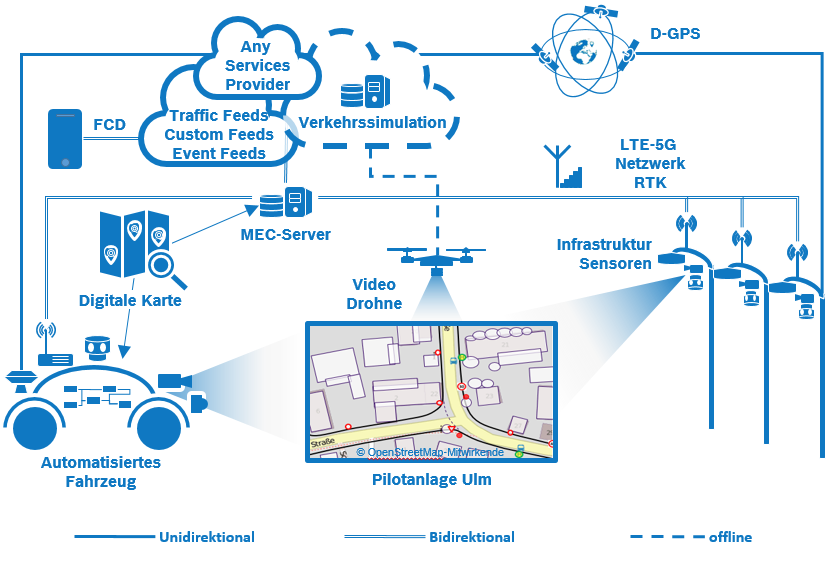
\includegraphics[width=\textwidth]{images/MECView_Arch_de_V1_mod.png}
	\caption[Übersicht über das Forschungsprojekt]{Übersicht über das Forschungsprojekt\protect\footnotemark}
\end{figure}
\footnotetext{Quelle: \url{https://www.uni-due.de/~hp0309/images/Arch_de_V1.png} (modifiziert)}

Diese Abschlussarbeit befasst sich mit dem Kommunikationsserver von \gls{mec}-View.
Das \gls{mec}-View Projekt wird durch das \gls{bmwi} gefördert und befasst sich mit der Thematik hochautomatisierter Fahrzeuge.
Es soll erforscht werden, ob und in wie weit eine durch externe Sensorik geleistete Unterstützung nötig und möglich ist, um in eine Vorfahrtstraße automatisiert einzufahren.

Das Forschungsprojekt ist dabei ein Zusammenschluss mehrerer Unternehmen mit unterschiedlichen Themengebieten.
Die IT-Designers Gruppe beschäftigt sich mit der Implementation des Kommunikationsservers, der auf der von Nokia zur Verfügung gestellten Infrastruktur im 5G Mobilfunk als \gls{mec} Server betrieben wird.
Erkannte Fahrzeuge und andere Verkehrsteilnehmer werden von den Sensoren von Osram via Mobilfunk an den Kommunikationsserver übertragen.
Der Kommunikationsserver stellt diese Informationen dem Fusionsalgorithmus der Universität Ulm zur Verfügung und leitet das daraus gewonnene Umfeldmodell an die hochautomatisierten Fahrzeuge von Bosch und der Universität Ulm weiter.
Durch hochgenaue, statische und dynamische Karten von TomTom und den Fahrstrategien von Daimler soll das Fahrzeug daraufhin automatisiert in die Kreuzung einfahren können.

%\subsection{Ablauf}
%Externe Sensoren übermitteln erkannte Fahrzeuge via Mobilfunk an einen \gls{mec}-Server, der direkt am Empfängerfunkmast angeschlossen ist. \todo{platform, vm?}
%Nachdem die erkannten Fahrzeuge der verschiedenen Sensoren zusammengeführt wurden (Fusions-Algorithmus), sollen sie an das autonom fahrende Fahrzeug über Mobilfunk übermittelt werden.
%Somit erhält das Fahrzeug bereits im Voraus Einsicht über eventuelle Möglichkeiten in die Vorfahrtsstraße einzufahren und könnte deshalb beispielsweise die Geschwindigkeit anpassen.
%Zudem sollen bei unübersichtlichen Kreuzungen somit zuverlässiger andere Verkehrsteilnehmer erkannt werden.


\section{Zielsetzung}

\todo{Dausmann \enquote{Sagen Sie doch zuerst, daß es schon was gibt}}

Das Ziel ist es, eine alternative Implementierung des \gls{mec}-View Servers in Rust zu schaffen.
Durch die Garantien (\autoref{rust:guarantees}) von Rust wird erhofft, dass der menschliche Faktor als Fehlerquelle gemindert und somit eine fehlertolerantere und sicherere Implementation geschaffen werden kann.

Eine Ähnlichkeit in Struktur und Architektur zu der bestehender C++ Implementation ist explizit nicht vonnöten.
Eventuelle Spracheigenheiten und einzigartige Features von Rust sollen im vollen Umfang genutzt werden können, ohne durch auferzwungene und unpassende Architekturmuster benachteiligt zu werden.
Es ist erwünscht, eine kompetitive Implementation in Rust zu schaffen.


\section{Aufbau der Arbeit}

Diese Arbeit ist im Wesentlichen in die folgenden Themengebiete aufgeteilt: Grundlagen, Anforderungs- und Systemanalyse, Systementwurf und Implementation und Auswertung.

Im Themengebiet Grundlagen sollen wesentliche Bestandteile dieser Arbeit erläutert und erklärt werden.
Hierzu zählt zum einen die Programmiersprache Rust in ihrer Entstehungsgeschichte, Garantien  und Sprachfeatures  (\autoref{rust}).
Zum anderen geht es um die hochperformante, serverbasierte Kommunikationsplattform mit ihren Protokollen (\autoref{com_plattform}) und dem Systemkontext, in dem diese betrieben wird.

In der Anforderungs- und Systemanalyse wird der Kontext, in dem der Server betrieben werden soll, genauer betrachtet. Umzusetzende funktionale und nicht-funktionale Anforderungen werden aufgestellt, sowie eine Übersicht über die Systeme geben, mit denen der Server interagiert wird.

Das Themengebiet Systementwurf und Implementation befasst sich mit dem theoretischen und praktischen Lösen der im vorherigen Kapitel aufgestellten Anforderungen. Aufgrund der Tatsache, dass es sich hierbei
um eine alternative Implementation handelt, wird zur bestehenden C++ Implementation Bezug genommen.
Architektonische Unterschiede im Systementwurf, die sich aufgrund von Sprach- und Bibliotheksunterschiede ergeben, werden hier genauer beschrieben.

Zuletzt wird eine Auswertung der Implementation aufgezeigt.

\todo{entsprechend zu aktualisieren}
	
\chapter{Die Programmiersprache Rust}
\label{rust}

%Rust ist eine Programmiersprache, die versucht performante -- und daher durch Abstraktionen mit keinem zusätzlichen \enquote{Kosten} \todo{ref zero cost abstractions} -- und sichere Programmierung zu ermöglichen.
Rust hat als Ziel, eine sichere (siehe \autoref{rust:guarantees}) und performante Systemprogrammiersprache zu sei.
Abstraktionen sollen die Sicherheit, Lesbarkeit und Nutzbarkeit verbessern aber keine unnötigen Performance-Einbußen verursachen (siehe \autoref{rust:zero_cost}).

Aus anderen Programmiersprachen bekannte Fehlerquellen -- wie vergessene \ccinline{NULL}-Pointer Prüfung, vergessene Fehlerprüfung, \enquote{dangling pointers} oder \enquote{memory leaks} --  werden durch strikte Regeln und mit Hilfe des Compilers verhindert (\autoref{rust:guarantees}).
Im Gegensatz zu Programmiersprachen, die dies mit Hilfe ihrer Laufzeitumgebung\footnote{u.a. Java Virtual Maschine (JVM), Common Language Runtime (CLR)} sicherstellen, werden diese Regeln in Rust durch eine statische Lebenszeitanalyse (\autoref{rust:static_analysis}) und mit dem Eigentümerprinzip (\autoref{rust:ownership}) bei der Kompilation überprüft und erzwungen.
%\todo{Anderswo als Best Practice Vorschläge, hier in Regeln erzwungen, ändert nicht viel, erzwingt nur korrekte programmierung}
Dadurch erreicht Rust eine zur Laufzeit hohe Ausführgeschwindigkeit.

Das Eigentümerprinzip (siehe \autoref{rust:ownership}) und die Markierung von Datentypen durch Merkmale (siehe \autoref{rust:traits}) vereinfacht es zudem, nebenläufige und sichere Programme zu schreiben.

Rust hat in den letzten Jahren viel an Beliebtheit gewonnen und ist 2018 das dritte Jahr in Folge als die beliebteste Programmiersprache in einer Umfrage auf Stack Overflow gewählt worden \cite{rust:stack_overflow:mose_loved}.
%Rust scheint dem Anspruch, eine sichere und performante Programmiersprache zu sein, gerecht zu werden:
Die Programmiersprache scheint den sich selbst gesetzten Zielen, performant und sicher zu sein, gerecht zu werden:

\begin{quotation}
	\textit{\enquote{Again, Rust guides you toward good programs}}
	\cite[497]{rust:orly_programming}
\end{quotation}

\begin{quotation}
	\textit{\enquote{[..]Leute, die [..] sichere Programmierung haben wollen, [..] können das bei Rust haben, ohne [..] undeterministischen Laufzeiten oder Abstraktionskosten schlucken zu müssen. }}
	\cite[Felix von Leitner in einem Blogeintrag]{rust:fefe}
\end{quotation}

\begin{quotation}
	\textit{\enquote{[..] Rust makes it safe, and  provides nice tools}} 
	\cite[Folie 130, Federico Mena-Quintero in \enquote{Ersetzen von C Bibliotheken durch Rust}]{rust:c_is_hostile_mena}
\end{quotation}

\begin{quotation}
	\textit{\enquote{Rust hilft beim Fehlervermeiden}} 
	\cite[Federico Mena-Quintero in einem Interview]{rust:c_is_hostile_golem}
\end{quotation}

\begin{quotation}
	\textit{\enquote{Rust is [..] a language that cares about very tight control}}
	\cite[Diskussion zwischen Programmierern auf Reddit]{rust:tight_control}
\end{quotation}


%Durch Merkmale (siehe \autoref{rust:traits}) kann die Zugriffsart auf Datentypen über verschiedene Threads hinweg festgelegt oder verhindert werden, wodurch falsche nebenläufige Programmierung zur Compilezeit erkannt und verhindert wird.
%Dies begünstigt parallelisierte Architekturen und ermöglicht es, die vielen CPU-Kerne auf modernen Computern einfacher zu nutzen.
%\todo{rust performance very wow, much parallel, great safety}

%Programmierer müssen sich für Rust an ein striktes Regelwerk und einen \enquote{besorgten} Compiler (siehe \autoref{rust:worried_compiler}) gewöhnen, erhalten im Gegenzug aber eine Sprache, die ein undefiniertes Verhalten nur in absoluten Ausnahmefällen kennt (siehe \autoref{rust:undefined}).
%Eine vom Compiler bemängelte Formatierung des Programmcodes und Benennung von Datentypen, Felder und Funktionen (siehe \autoref{rust:styleguide}) erlaubt ein einheitliches Auftreten des Programmcodes innerhalb der \todo{Community}.

%\todo{rust sehr sauber, nahezu nix undefined (ref), nix uninitalized access(ref), datentypen namen u/i..(ref), styleguide}


\clearpage
\section{Geschichte}
\label{rust:history}

In 2006 begann Graydon Hoare die Programmiersprache Rust in seiner Freizeit als Hobbyprojekt zu entwickeln \cite{rust:faq}.
Als Grund nannte er seine Unzufriedenheit mit der Programmiersprache C++, in der es sehr schwierig sei, fehlerfreien, speichersicheren und nebenläufigen Programmcode zu entwickeln.
Zudem beschrieb er C++ als \enquote{ziemlich fehlerträchtig} \cite{rust:heise_interview_graydon}.

Auch Federico Mena-Quintero -- Mitbegründer des GNOME-Projekts \cite{rust:gnome:federico}  --
äußerte in einem Interview mit Golem im Juli 2017 seine Bedenken an der Verwendung der \enquote{feindseligen} Sprache C \cite{rust:c_is_hostile_golem}.
In Vorträgen vermittelt er seither, wie Bibliotheken durch Implementationen in Rust ersetzt werden können \cite{rust:c_is_hostile_mena}.

Ab 2009 begann Mozilla die Weiterentwicklung finanziell zu fördern, als mit einfachen Tests die Kernprinzipien demonstriert werden konnten.
Die Entwicklung der Programmiersprache, des Compilers, des Buchs, von Cargo, von crates.io und von weiteren Bestandteilen findet öffentlich einsehbar auf \gls{github}  unter \url{https://github.com/rust-lang} statt.
Dadurch kann sich jeder an Diskussionen oder Implementation beteiligen, seine Bedenken äußern oder Verbesserungen vorschlagen.

Durch automatisierte Tests (siehe \autoref{rust:tests}) in Kombination mit drei Veröffentlichungskanälen (\enquote{release}, \enquote{stable} und \enquote{nightly}) und \enquote{feature gates} (siehe \autoref{rust:feature_gates}) wird die Stabilität des Compilers und die der Standardbibliothek (\autoref{rust:stdlib}) gewährleistet.

Rust ist wahlweise unter MIT oder der Apache Lizenz in Version 2 verfügbar \cite{rust:copyright}.

\section{Anwendungsgebiet}

Das Ziel von Rust ist es, das Designen und Implementieren von sicheren und nebenläufigen Programmen möglich zu machen.
Gleichzeitig soll der Spagat geschaffen werden, nicht nur ein sicheres aber lediglich theoretisches Konstrukt zu sein, sondern  in der Praxis anwendbar zu sein.
Als Beweis könnte hierbei auf die Umstellung von Firefox auf Rust und Servo -- ein minimaler Webbrowser komplett in Rust geschrieben -- verwiesen werden \cite{rust:faq}.

Interessant ist eine Diskussion von 2009, bei der \enquote{sicher aber nutzlos} und \enquote{unsicher aber brauchbar} gegenübergestellt wurde.
Programmiersprachen scheinen auf der Suche nach dem nicht existierende \enquote{Nirvana} zu sein, das sowohl sichere als auch brauchbare Programmierung verspricht \cite[ab ca Minute 58:20]{rust:infoq:null}.
Rust möchte dieses Nirvana gefunden haben.
% bei einer Diskussion \footnote{Siehe auch \enquote{unsafe but useful}/\enquote{safe but useless} \cite[ab ca Minute 58:20]{rust:infoq:null}}.

\subsection{Kompatibilität}
Da Rust den \gls{llvm}-Compiler nutzt, erbt Rust auch eine große Anzahl der Zielplattformen die \gls{llvm} unterstützt.
Die Zielplattformen sind in drei Stufen unterteilt, bei denen verschieden stark ausgeprägte Garantien vergeben werden. Es wird zwischen
\begin{itemize}
	\item \enquote{Stufe 1: Funktioniert garantiert} (u.a. X86, X86-64),
	\item \enquote{Stufe 2: Compiliert garantiert} (u.a. ARM, PowerPC, PowerPC-64) und
	\item \enquote{Stufe 3} (u. a. Thumb (Cortex-Microcontroller))
\end{itemize}
unterschieden \cite{rust:platform_support}.
Diese Unterscheidung wirkt sich auch auf die Stabilisierungsphase und Implementation neuer Funktionen aus (Beispiel \enquote{128-bit Integer Support} \cite{rust:github:128bit_integer}).

\subsection{Veröffentlichungszyklus}
\label{rust:feature_gates}

Es stehen Versionen in drei verschieden Veröffentlichungskanälen zur Verfügung:
\begin{itemize}
	\item \textbf{nightly}:
	Version, die einmal am Tag mit dem aktuellen Stand des Quellcodes gebaut wird.
	Experimentelle und nicht fertige Features sind hier zwar enthalten, aber hinter \enquote{feature gates} versteckt.
	Diese \enquote{Tore} können durch entsprechende Anmerkungen (siehe \autoref{rust:annotations}) geöffnet werden.%, so ermöglicht (\rustcinline{#[feature(const_fn)]} die Definition von konstanten Funktionen (Stand \today).
	
	\item \textbf{beta}: Alle sechs Wochen wird die aktuellste Nightly zur Beta befördert und es werden nur noch Fehler aus dieser Version getilgt.
	Dieser Prozess könnte auch als Reifephase bezeichnet werden.
	\item \textbf{stable}: Nach sechs Wochen wird die aktuellste Beta zur Stable befördert und veröffentlicht.
	Gleichzeitig wird auch eine neue Beta veröffentlicht.
\end{itemize}

\subsection{Ökosystem}

Mit Rust wird nicht nur eine Programmiersprache, sondern auch ein umfassendes Ökosystem angeboten.

Cargo ist hierbei vermutlich das größte angebotene Werkzeug.
Es löst Abhängigkeiten auf, indem es auf das öffentliche Verzeichnis unter \url{https://crates.io} zurückgreift und diese entsprechend herunterlädt und compiliert.
Zum jetzigen Zeitpunkt (\today) sind über 14.000 Crates öffentlich erreichbar und nutzbar.
%Zudem wird bei der Nutzung von Cargo eine \textit{Cargo.toml} verlangt, in der Metainformationen einer Crate hinterlegt sind.
%Dies umfasst u.a. Name, Version, Autor, Lizenz und Abhängigkeiten.

Eine Crate kann von jedem veröffentlicht werden, insofern derjenige ein \gls{github}-Konto besitzt, der Name der Crate noch nicht vergeben ist und der Programmcode compiliert.
Die API-Dokumentation der jeweiligen Crate wird dabei automatisiert auf \url{https://docs.rs} veröffentlicht.

Unter \url{https://www.rust-lang.org} ist die Website von Rust erreichbar und unter \url{https://doc.rust-lang.org} sowohl die API-Dokumentation der Standardbibliothek als auch das hauseigene Rust Buch in Version 1 und 2.
Die Entwicklung findet dagegen auf \gls{github} unter \url{https://github.com/rust-lang} statt.

\todo{..}
Neue Bibliotheken für die Standardbibliothek werden zuerst unter \url{https://github.com/rust-lang-nursery} entwickelt.
Die Entwicklung und Diskussionen hierzu können so ungestört stattfinden, ohne sich an das offizielle und \todo{bürokratische} Vorgehen \todo{via RFCs} zu halten (\todo{wie unter rust-lang üblich}).
Nach einer Bewährungsprobe können diese Crates nach \url{https://github.com/rust-lang} und letztendlich in die Standardbibliothek übernommen werden \cite{rust:internals:1242_Recap}.

\todo{..}
Unter \url{https://internals.rust-lang.org/} finden interne Diskussionen zu fundamentalen Herangehensweisen und Philosophien der Kernentwickler statt.


Kleine Testprogramme und Experimente können auf dem \enquote{Spielplatz} unter \url{https://play.rust-lang.org} compiliert und ausgeführt werden, ohne lokal etwas zu installieren.

\todo{rustup.rs}

\section{Aufbau eines Projektverzeichnisses}

Der Aufbau eines Rust Projektverzeichnis ist auf zwei verschiedene Arten möglich.
Zum einen gibt es den klassische Aufbau, in dem lediglich der Programmcode liegt und der Compiler direkt aufgerufen und parametrisiert wird.
Zum anderen wird der Aufbau als Crate (siehe \autoref{rust:structure:crate}) empfohlen, da dadurch Abhängigkeiten automatisch aufgelöst werden können aber auch Metainformationen bezüglich des Autors, der Version und der Abhängigkeiten hinterlegt werden müssen.
Ein klassischer Aufbau ist nur selten anzutreffen.


\subsection{Klassisch}
\label{rust:structure:classic}
\begin{wrapfigure}{L}[-1em]{.5\textwidth}
	\rustcinclude
		{rust:structure:classi}
		{Verzeichnisstruktur des Quelltext-Verzeichnisses}
		{sections/rust.classic.txt}
\end{wrapfigure}

Das Quelldatei-Verzeichnis sollte entweder eine \textit{main.rs} für ausführbare Programme oder eine \textit{lib.rs} für Bibliotheken enthalten.
Während der Paketmanager Cargo eine solche Benennung als Standardkonvention erwartet, kann bei manueller Nutzung des Compilers auch ein anderer Name für die Quelldatei vergeben werden.

Der Compiler startet in der Wurzeldatei und lädt weitere Module, die durch \rustcinline{mod module;} gekennzeichnet sind (ähnlich \ccinline{#include "module.h"} in C/C++).
Ein Modul kann dabei eine weitere Quelldatei oder ein ganzes Verzeichnis sein.
Ein Verzeichnis wird aber nur als gültiges Modul interpretiert, wenn sich eine \textit{mod.rs}-Datei darin befindet.
Um Datentypen und Funktionen aus einem Modul nutzen zu können, ohne deren kompletten Pfad bei jeder Nutzung auszuschreiben, können sie durch zum Beispiel \rustcinline{use module::functionality::Data;} in dem aktuellen Namensraum bekannt gemacht werden.
Dies ähnelt einem \javacinline{import} aus Java oder einem \cscinline{using} aus C\#.

Wie bereits angedeutet, wird in Rust nicht eine \enquote{Klasse}, Datenstruktur oder Aufzählung pro Datei erwartet, sondern eine Quelldatei entspricht einem Modul.
Dieses umfasst in vielen Fällen wenige aber mehrere Datenstrukturen, zugehörige Aufzählungen und Fehlertypen.
%Module (Verzeichnisse oder Quelldateien) gesucht wird. , in der Module durch \rustcinline{mod module;} und Quelldateien durch \rustcinline{mod functionality;} \enquote{inkludiert} werden können.
%Eine Datei \textit{mod.rs} ist die Wurzeldatei eines Moduls.

\subsection{Als Crate}
\label{rust:structure:crate}

\begin{wrapfigure}{R}{.4\textwidth}
	\rustcincludeml
		{rust:structure:cargo}
		{Vereinfachte Verzeichnisstruktur einer \enquote{crate}}
		{sections/rust.cargo.txt}
\end{wrapfigure}



Eine \enquote{Crate} (dt. Kiste/Kasten) erweitert den klassischen Aufbau um eine \textit{Cargo.toml} Datei, in der Metainformationen zum Projekt hinterlegt werden.
Durch die Benutzung des Werkzeugs \enquote{Cargo} (dt. Fracht/Ladung) können Abhängigkeiten automatisch aufgelöst, heruntergeladen und compiliert werden.

Eine Crate kann entweder ein ausführbares Programm oder eine Bibliothek sein.
Davon abhängig ist die Wurzeldatei \textit{src/main.rs} (für ein ausführbares Programm) oder \textit{src/lib.rs} (für eine Bibliothek).
Mit dem Erzeugen einer Crate (\rustcinline{cargo new --bin meinProg} bzw. \rustcinline{cargo new --lib meineBib}) wird auch gleichzeitig \gls{git} für das Verzeichnis initialisiert.

\section{Hello World}


\begin{wrapfigure}{L}{.5\textwidth}
	\rustcinclude
		{rust:hello_world}
		{\enquote{Hello World} in Rust}
		{sections/rust.hello_world.rs}
\end{wrapfigure}

Der Programmcode in \autoref{rust:hello_world} gibt auf der Konsole \monospaceinline{Hello World} aus.
Dass \rustcinline{fn} die Funktion \rustcinline{main} definiert und diese der Startpunkt des Programms ist, wird vermutlich wenig überraschend sein.
Viel überraschender ist vermutlich eher das Ausrufezeichen in Zeile 2, da es auf den ersten Blick dort nicht hingehören sollte.
In Rust haben Ausrufezeichen und Fragezeichen besondere Bedeutungen, weswegen die Verwendung in Zeile 2 trotzdem richtig ist.

Die Bedeutung des Fragezeichens dient zum schnelleren Auswerten von \rustcinline{Rusult<_, _>}-Werten und wird in \autoref{rust:result} genauer erklärt.
Das Ausrufezeichen kennzeichnet, dass der ansonsten augenscheinliche Funktionsaufruf tatsächlich ein Aufruf einer Makrofunktion ist.

Eine Funktion \rustcinline{println} gibt es nicht, auch keine aus C erwarteten Funktionen wie \ccinline{printf}, \ccinline{fputs} oder \ccinline{sprintf}.
Eine Ausgabe erfolgt durch das \rustcinline{println!} Makro, welches einen \rustcinline{String} durch Nutzung des \rustcinline{format!} Makros erstellt und formatiert.
Daraufhin wird das \rustcinline{writeln!} Makro verwendet, um die formatierte Zeichenkette auf die Standardausgabe zu schreiben.

\section{Einfache Datentypen}
\label{rust:types:simple}

Die Datentypen in Rust sind im wesentlichen die üblichen  Verdächtigen: \rustcinline{bool} für boolische Ausdrücke; \rustcinline{char} für ein einzelnes Unicode Zeichen; \rustcinline{str} für eine Zeichenkette; \rustcinline{u8}, \rustcinline{i8}, \rustcinline{u16}, \rustcinline{i16}, \rustcinline{u32}, \rustcinline{i32}, \rustcinline{u64}, \rustcinline{i64}, (bald \rustcinline{u128}, \rustcinline{i128} \cite{rust:github:128bit_integer:rfc}) und \rustcinline{usize}, \rustcinline{isize}  für ganzzahlige Werte; \rustcinline{f32}, \rustcinline{f64} für Fließkommazahlen in einfacher und zweifacher Präzision; Arrays und Slices \cite{rust:book:primitives}.

Ganzzahlige Datentypen mit einem führenden \rustcinline{u} sind vorzeichenlos (\textit{unsigned}), vorzeichenbehaftete Datentypen (\textit{signed}) sind dagegen mit einem \rustcinline{i} gekennzeichnet.
Fließkommazahlen sind stattdessen mit einem führenden \rustcinline{f} (\textit{floating point}) gekennzeichnet.
Die darauf folgende Zahl gibt die Anzahl der Bits wieder, die für den Datentyp verwendet wird.
Die einzige Ausnahme sind die ganzzahligen Datentypen \rustcinline{usize} und \rustcinline{isize}, da diese immer so groß sind, wie die Architektur der Zielplattform.
Für die Indexierung eines Arrays oder einer Slice würden andere Datentypen, mit einer fest definierten Größe, keinen Sinn ergeben, da das Maximum an adressierbaren Elementen von der Architektur der Zielplattform abhängig ist.

Durch dieses Schema bei der Bezeichnung der Datentypen wird eine Verwirrung wie zum Beispiel in C unterbunden, wo die primitiven Datentypen (\ccinline{short}, \ccinline{int}, \ccinline{long}, ..) keine definierte Größe haben, sondern abhängig vom eingesetzten Compiler und der Zielplattform sind \cite[187]{deitel2013c}. Erst ab C99 wurden zusätzliche, aber optionale, ganzzahlige Datentypen mit festen Größe definiert \cite[141]{goll2014c}.

Konstanten können in Rust direkt einem Datentyp zugewiesen werden, indem dieser angehängt wird: \rustcinline{4711u16} ist vom Datentyp \rustcinline{u16}.
Unterstriche dürfen an beliebiger Stelle Ziffern trennen, um die Lesbarkeit zu erhöhen: \rustcinline{1_000_000_f32}.
Eine Schreibweise in Binär (\rustcinline{0b0000_1000_u8}), in Hexadezimal (\rustcinline{0xFF_08_u16}) oder in Oktal (\rustcinline{0o64_u8}) ist auch möglich. 
Konstante Zeichen und Zeichenketten können auch automatisch durch ein vorangestelltes \textit{b} in Bytes gewandelt werden: \rustcinline{b'b'} entspricht \rustcinline{0x62_u8} und \rustcinline{b"abc"} entspricht \rustcinline{&[0x61_u8, 0x62_u8, 0x63_u8]}.

Arrays haben immer eine zur Compilezeit bekannte Größe und müssen auch immer mit einem Wert initialisiert werden (siehe \autoref{rust:no_unitialized_usage}).
Dynamische Arrays auf dem Stack gibt es (noch? \cite{rust:github:alloca}) nicht,
stattdessen wird auf die Vektor Implementation der Standardbibliothek verwiesen (siehe \autoref{rust:stdlib}).
Die Notation für Arrays ist \rustcinline{[<Füllwert>; <Größe>]}, wobei die Größe ein konstanter Wert sein muss.
\rustcinline{[0_u8; 128]} steht demnach für ein 128 Byte langes Array mit Werten vom Datentyp \rustcinline{u8}, das mit 0-en initialisiert ist.

\enquote{Slices} (dt. Scheiben/Stücke) bezeichnet in Rust Referenzen auf Arrays oder auf Teilbereiche von Arrays und Slices.
In einem so genannten \enquote{fat pointer} wird der Startpunkt und die Größe der Slice gespeichert  (siehe auch \autoref{rust:memory_layout:vec_slice} auf Seite \pageref{rust:memory_layout:vec_slice}).
Hierdurch kann ein Zugriff außerhalb den Grenzen einer Slice oder eines Arrays verhindert werden, %, oder, falls möglich, zur Compilezeit verhindern.% (siehe \autoref{rust:zero_cost}).
ein Buffer-Overflow ist in Rust daher nicht möglich.

Die Notation einer Slice ähnelt der eines Arrays: \rustcinline{&[<Datentyp>]}.
Eine Slice kann zudem immer nur über eine eine Referenz angesprochen werden (siehe \autoref{rust:reference}).
Um eine Slice auf ein Array oder eine andere Slice zu erhalten, muss der Start- und  Endindex des Teilbereiches angegeben werden.
Falls kein Start- oder Endindex angegeben wird, wird das jeweilige Limit übernommen.


Folgendes Beispiel soll die Notation von Arrays und Slices verdeutlichen:

\rustcinclude
	{rust:slices:example}
	{Beispiel eines Arrays und einer Slice}
	{sections/rust.slices.rs}
	
Das in \autoref{rust:slices:example} gezeigte Programm, gibt auf der Konsole \rustcinline{2, 3, 4, } aus.

Variablen werden durch das \rustcinline{let} Schlüsselwort gebunden, das heißt, der Variable wird die Eigentümerschaft für den Wert zugewiesen.
Ausnahmen können Datentypen mit dem Merkmal \rustcinline{Copy} bilden, da diese ein implizite Kopie erlauben (siehe \autoref{rust:generics}).
Anstatt eine Variable optional als unveränderlich zu kennzeichnen (\ccinline{const} in C, \javacinline{final} in Java), wird eine Variable in Rust optional als veränderlich gekennzeichnet (\rustcinline{mut}). Standardmäßig ist eine Variable unveränderlich.

\subsubsection{Lokale Typinferenz}

Da Rust ein statisches Typensystem mit lokaler Typinferenz besitzt, muss der Datentyp einer Variable nicht notiert werden, sondern können automatisiert erkannt werden.
Dies gilt aber nur lokal, also innerhalb von Funktionen und Closures.
Parameterlisten und Rückgabewerte von Funktionen müssen die Datentypen explizit angegeben (siehe \autoref{rust:fn}).

\rustcinclude
	{rust:type_interference}
	{Beispiel für lokale Typinferenz}
	{sections/rust.type_interference.rs}
	



\section{Zusammengesetzen Datentypen}
\label{rust:types:composed}

Die Programmiersprache Rust kennt neben den einfachen Datentypen (\autoref{rust:types:simple}) weitere Möglichkeiten Daten zu organisieren:
\begin{itemize}
	\item ein Tupel, das mehrere Werte namenlos zusammenfasst: \rustcinline{(f32, u8)}: \rustcinline{a.0 = 1.0_f32},
	\item eine Datenstruktur, die wie in C Datentypen namenbehaftet zusammenfasst: \linebreak\rustcinline{struct Punkt \{ x: f32, y: f32 \} }: \rustcinline{p.x = 1.0_f32},
	\item und Aufzählungen: \rustcinline{enum Bildschirm \{ Tv, Monitor, Leinwand \}}.
\end{itemize}

Im Vergleich zu C kann ein Eintrag in einem \rustcinline{enum} gleichzeitig Daten wie eine Datenstruktur oder ein Tupel halten, oder lediglich einen Ganzzahlwert repräsentieren.

Mit dem \rustcinline{type} Schlüsselwort können Aliase erstellt oder im Falle von FFI (siehe \autoref{rust:ffi}) aufgelöst werden: \rustcinline{type Vektor = (f32, f32);}
Felder einer Struktur können zudem mit \rustcinline{pub} oder \rustcinline{pub(crate)} gekennzeichnet werden (siehe \autoref{rust:access_modifier}).

Seit Version 1.19 ist auch der Datentyp \rustcinline{union} in Rust verfügbar \cite{rust:v1.19}.
Eine \rustcinline{union} kann aber nur in \rustcinline{unsafe}-Blöcken verwendet werden, da der Compiler eine ordnungsgemäße Nutzung nicht überprüfen kann.
Für diese Abschlussarbeit hat der Datentyp aber keine Relevanz und wird daher nicht weiter erwähnt.

\subsubsection{Referenzen}
\label{rust:reference}

Auf alle Datentypen können Referenzen erstellt werden, um auf diese zuzugreifen, ohne sie zu konsumieren.
In Rust spricht man dann oft davon, den Wert zu \enquote{leihen}, da sich der Eigentümer nicht ändert, sondern für den Gültigkeitsbereich der Referenz eine andere Variable auf den Wert verweist.
Wie bei Variablen, wird zwischen Referenzen auf unveränderlichen und veränderlichen Werte unterschieden (siehe \autoref{rust:ownership}).
Die Notation für Referenzen auf unveränderliche Werte ist \rustcinline{&<Datentyp>}.
Erwartungsgemäß ist \rustcinline{&mut <Datentyp>} die Notation für Referenzen auf veränderliche Werte.
Referenzen auf Referenzen sind möglich.
Eine manuelle Dereferenzierung einer Referenz ist in den allermeisten Fällen nicht nötig, sondern wird vom Compiler vorgenommen.
In Fällen, in denen dies nicht wie erwartet automatisch geschieht, kann eine manuelle Dereferenzierung durch den \rustcinline{*}-Operator erzwungen werden.

\section{Funktionen, Ausdrücke und Statements}
\label{rust:fn}

Funktionen werden durch \rustcinline{fn} gekennzeichnet, gefolgt von dem Funktionsnamen, der Parameterliste und zuletzt der Datentyp für den Rückgabewert.
Selbst wenn kein expliziter Rückgabetyp angegeben wird, wird formal \rustcinline{()} zurück gegeben; \rustcinline{()} entspricht etwa \ccinline{void} aus bekannten Programmiersprachen.
Die Parameterliste unterscheidet sich von bekannten Programmiersprachen wie C und Java, indem zuerst der Variablenname und darauf folgend der Datentyp notiert wird.

\rustcinclude
	{rust:fn:add}
	{Beispiel einer Funktion}
	{sections/rust.fn.add.rs}
	
Obwohl in Zeile 2 von \autoref{rust:fn:add} kein \rustcinline{return} zu sehen ist, wird trotzdem das Ergebnis der Addition zurückgegeben.
Dies liegt daran, dass in Rust vieles ein Ausdruck ist und somit einen Rückgabewerte liefert \cite{rust:book:statements}.
Auch ein if-else ist ein Ausdruck und kann einen Rückgabewert haben.
Ein bedingter Operator (?:) is somit unnötig, da stattdessen ein if-else verwendet werden kann: \rustcinline{let a = if b \{ c \} else \{ d \};}.



\section{Implementierung einer Datenstruktur}

Zu einer Datenstruktur oder Aufzählung kann ein individuelles Verhalten implementiert werden.
In dieser Kombination ähneln diese Konstrukte sehr einer Klasse aus bekannten objektorientierten Programmiersprachen, wie zum Beispiel Java, C\# oder C++ (siehe auch \autoref{rust:oop}).

Einen Konstruktor gibt es jedoch nicht; lediglich die Konvention, eine statische Funktion \rustcinline{new} stattdessen zu verwenden \cite{rust:book:constructors}:

\rustcinclude
	{rust:struct:impl}
	{Punkt Datenstruktur mit einem \enquote{Konstruktor}}
	{sections/rust.struct.impl.rs}
	
Manchmal wird auch \rustcinline{Default} implementiert (siehe \autoref{rust:trait:default}), wodurch eine statische Funktion \rustcinline{default()} als Konstruktor ohne Parameter bereitgestellt wird.

Da eine Funktionsüberladung nicht möglich ist, sollen stattdessen sprechende Name verwendet werden.
Der \rustcinline{Vec<_>} der Standardbibliothek (siehe \autoref{rust:stdlib}) bietet zum Beispiel zusätzlich \rustcinline{Vec::with_capacity(capacity: usize)} an, um einen Vektor mit einer bestimmten Kapazität zu initialisieren.

Funktionen die sich auf eine Instanz beziehen, haben als ersten Parameter die Variable \rustcinline{self} (konsumierend), \rustcinline{&self} (lesend leihend) oder \rustcinline{&mut self} (exklusiv leihend) deklariert.
Die \rustcinline{self}-Variable entspricht dabei dem \javacinline{this} aus C++, C\# oder Java:
\rustcinline{fn x_eq_y(&self) -> bool \{ self.x == self.y \}}.
Ein großgeschriebenes \rustcinline{Self} bezieht sich auf den eigenen Typ, deshalb könnte die Funktion aus \autoref{rust:struct:impl} auch folgende Signatur haben: \rustcinline{pub fn new(x: f32, y: f32) -> Self ...}.
Dies ist aber selten und oft nur in generischem Code anzutreffen (siehe \autoref{rust:traits}).

Für Funktionen können auch die Zugriffsmodifikatoren festgelegt werden (siehe \autoref{rust:access_modifier}).

\section{Generalisierung durch Traits}
\label{rust:traits}
\label{rust:generics}
\label{rust:trait:default}

Ähnlich wie Java oder C\# bietet Rust durch einen eigenen Typ die Möglichkeit, ein gewünschtes Erscheinungsbild zu generalisieren, ohne gleichzeitig eine Implementation vorzugeben.
Im Rust wird dieser Typ \enquote{Trait} (dt. Merkmal) genannt.

Für Merkmale werden Funktionen in einem entsprechenden \rustcinline{trait <Name> \{ \}}-Block ohne Rumpf deklariert.
Optional kann auch ein Standardrumpf implementiert werden, der bei einer Spezialisierung überschrieben werden darf.
Auch auf ein Merkmal kann ein Zugriffsmodifikator gesetzt werden (siehe \autoref{rust:access_modifier}).

Die Implementation eines Merkmals wird für jeden Datentyp in einem separaten Codeblock vorgenommen und entspricht der Notation \rustcinline{impl Merkmal for Datentyp \{ fn ... \} }.
Alternativ können Implementationen auch für ganze Gruppen von anderen Merkmalen vorgenommen werden: \rustcinline{impl<T> Merkmal for T where T: Clone \{ ... \} } (entspricht: \enquote{implementiere \rustcinline{Merkmal} für all die, die \rustcinline{Clone}-bar sind}).

In Zukunft -- oder jetzt in \enquote{nightly} und hinter dem \enquote{feature gate} \rustcinline{specialization} -- wird es möglich sein, ein Standardverhalten für Gruppen zu implementieren und dieses, für einen speziellen Typ, zu überschreiben \cite{rust:github:specialization}.

Merkmale unterscheiden sich in ihrer Handhabung gegenüber anderen Datentypen, da sie im Allgemeinen keine bekannte Größe zur Compilezeit haben.
Während dies in Programmiersprachen wie Java und C\# automatisch durch die Darstellung abstrahiert und versteckt wird, hat ein Entwickler in Rust mehr Kontrolle über die Handhabung.

Dabei gibt es mehrere Vorgehensweisen:
\begin{itemize}
	\item Die einfachste Art erfolgt über das Leihen mittels Referenz: \rustcinline{fn foo(bar: \&Bar)} oder \rustcinline{fn foo(bar: \&mut Bar)} -- ein Unterschied zu anderen Datentypen ist nicht zu erkennen.
	Hierbei werden Funktionen aber dynamisch über eine \enquote{vtable} aufgerufen, weswegen dies höhere Laufzeitkosten mit sich bringt.
	In Zukunft soll dieser Syntax eventuell durch \rustcinline{fn foo(bar: \&dyn Bar)} und \rustcinline{fn foo(bar: \&mut dyn Bar)} ersetzt werden, um deutlicher auf den dynamischen Aufruf hinzuweisen \cite{rust:github:dyn}.
	
	\item Alternativ kann das Objekt, das das geforderte Merkmal implementiert, auf den Heap verschoben und anschließend davon die Eigentümerschaft übertragen werden.
	Dies ist möglich, da das Verschieben auf den Heap die Größe der \rustcinline{Box} nicht beeinflusst.
	Eine \rustcinline{Box} ist letztendlich nur ein Pointer auf einen Speicherbereich auf dem Heap.
	Ein Merkmal in einer \rustcinline{Box} wird \enquote{Trait-Object} genannt und eine Funktionsdeklaration könnte so aussehen: \rustcinline{fn foo(bar: Box<Bar>)}.
	
	\item Die performanteste Alternative ist eine spezialisierte Funktion.
	Der Compiler dupliziert automatisch für jeden Datentyp die Funktion, setzt diesen ein und führt Optimierungen für den jeweiligen Datentyp durch (ähnlich einer Templateklasse in C++).
	In der Notation wird ein lokaler Typ deklariert, der als Bedingung ein oder mehrere Merkmale implementiert haben muss: \rustcinline{fn foo<T: Bar>(bar: T)}.
\end{itemize}

Eine Deklaration \rustcinline{fn foo(bar: Bar)} für das Merkmal \monospaceinline{Bar} ist nicht möglich, da zur Compilezeit eine eindeutige Größe nicht bekannt ist.
Der zu reservierende Speicher für die Variable kann nicht bestimmt werden, weswegen eine Übergabe über den Stack nicht möglich ist.


Im Folgenden werden oft anzutreffende und wichtige Merkmale aus der Standardbibliothek kurz erläutert:
\begin{itemize}
	\item \monospaceinline{Send}: Markiert einen Datentyp als zwischen Threads übertragbar. Automatisch für alle Datentypen implementiert, bei denen auch alle beinhalteten Datentypen von Typ Send sind. Manuelle Implementation ist nicht sicher \cite{rust:book:send_sync}.
	
	\rustcinline{!Send} verhindert dagegen, dass ein Wert zu anderen Threads übertragen werden darf.
	Somit können ansonsten rein textuell beschriebene Beschränkungen, wie zum Beispiel für der OpenGL-Kontext, durch den Compiler überprüft und erzwungen werden.
	
	\item \monospaceinline{Sync}: Markiert einen Datentype als zwischen Threads synchronisierbar, d.h. mehrere Threads dürfen gleichzeitig lesend darauf zugreifen.
	\rustcinline{!Sync} verbietet dies hingegen.
	Automatisch für alle Datentypen implementiert, bei denen auch alle beinhalteten Datentypen von Typ \rustcinline{Sync} sind. Manuelle Implementation ist nicht sicher \cite{rust:book:send_sync}.
	
	\item \monospaceinline{Sized}: Verlangt eine zur Compilezeit bekannte Größe. \monospaceinline{?Sized} erlaubt dagegen eine unbekannte Größe zur Compilezeit.
	
	\item \monospaceinline{Copy}: Markiert einen Datentyp, der durch einfaches Speicherkopieren (etwa \enquote{memcpy}) vervielfacht werden kann. Verlangt, dass alle beinhalteten Datentypen auch \monospaceinline{Copy} sind.
	Alle einfachen Datentypen sind bereits \monospaceinline{Copy}.
	
	\item \monospaceinline{Clone}: Markiert einen Datentyp, der vervielfacht werden kann, dies jedoch nicht durch Kopieren des Speichers möglich ist -- zum Beispiel da der Referenzzähler von \rustcinline{Arc} oder \rustcinline{Rc} erhöht werden muss.
	Stellt die Funktion \rustcinline{clone} bereit, die dafür explizit aufgerufen werden muss.
	Verlangt für eine automatisierte Implementation, dass alle beinhalteten Datentypen auch \monospaceinline{Clone} sind.
	Alle einfachen Datentypen sind bereits \monospaceinline{Clone}.
	
	\item \monospaceinline{Debug} und \monospaceinline{Display}: Erzwingt die Implementation von Funktionen, um einen Datentyp als Text darzustellen. Entweder mit möglichst vielen Zusatzinformationen (\monospaceinline{Debug}) oder schön (\monospaceinline{Display}).
	Verlangt für eine automatisierte Implementation, dass alle beinhalteten Datentypen auch \monospaceinline{Debug} bzw \monospaceinline{Display} sind.
	
	\item \monospaceinline{Default}: Erzwingt die Implementation einer statische Methode \monospaceinline{default()}, die wie ein leerer Standardkonstruktor von Java oder C\# wirkt: Erzeugung einer neuen Instanz mit Standardwerten.
	Verlangt für eine automatisierte Implementation, dass alle beinhalteten Datentypen auch \monospaceinline{Default} sind.
	
	\item \rustcinline{PartialEq}: Verlangt die Implementation einer Funktion, um mit Instanzen des gleichen Typs verglichen werden zu können.
	Im Vergleich zu \monospaceinline{Eq} erlaubt \monospaceinline{PartialEq}, dass Typen keine volle Äquivalenzrelation haben.
	Dies ist zum Beispiel für den Vergleich von Fließkommazahlen wichtig, da laut IEE754  \rustcinline{Nan} ungleich zu allem ist, auch zu sich selbst (\rustcinline{Nan != Nan}) \cite{wiki:nan}\cite[272-275]{rust:orly_programming}\cite{rust:doc:partialeq}.
	
	\item \rustcinline{Eq}: Erlaubt dem Compiler einen Vergleich auf Bit-Ebene durchzuführen, ungeachtet des Datentyps \cite{rust:doc:eq}.
	
	\item \rustcinline{PartialOrd}: Verlangt die Implementation einer Funktion, damit Instanzen des gleichen Typs sortiert werden können. Erlaubt aber auch, dass Werte zueinander nicht sortierbar sind.
	Dies ist zum Beispiel für Fließkommazahlen wichtig, da laut IEE754  \rustcinline{Nan} nicht sortiert werden kann (weder \rustcinline{Nan <= 0} noch \rustcinline{Nan > 0} ergibt \rustcinline{true}) \cite{wiki:nan}\cite[275-277]{rust:orly_programming}\cite{rust:doc:partialord}.
	
	\item \rustcinline{Ord}: Erzwingt im Gegensatz zu \rustcinline{PartialOrd}, dass Werte zueinander immer geordnet werden können.
	
	\item \monospaceinline{Drop}: Verlangt die Implementation einer Funktion, die kurz vor der Speicherfreigabe eines Objekts aufgerufen wird (ähnlich Destruktor aus C++).
\end{itemize}

Mit der Anmerkung \rustcinline{#[derive(..)]} ist eine automatisierte Implementation genannter Merkmale oft möglich, insofern die jeweiligen Bedingungen erfüllt sind.
So kann im allgemeinen \rustcinline{#[derive(Clone)]} genutzt werden, um eine Datenstruktur oder eine Aufzählung automatisch klonbar zu machen oder \rustcinline{#[derive(Debug)]}, um automatisch alle Felder in Text wandeln zu können.
Ein ergonomisches aber auch Fehler reduzierendes Feature.
%Dadurch wird der menschliche Faktor als Fehlerquelle für oft genutzte aber im Prinzip einfache Mechanismen ausgeschlossen.

\subsection{Closure}
\label{rust:closures}

\todo{..}
Mit Closures bietet Rust einen entsprechenden Sprachkonstrukt um Lambdas wie in Programmiersprachen wie Java, JavaScripit, C\# und C++ darstellen zu können.
Übergabeparameter befinden sich in der Notation zwischen zwei senkrechten Strichen, deren Typ nicht explizit angegeben werden müssen, da der Compiler diese meist ableiten kann.
In geschweiften klammern ist anschließend der Rumpf zu finden.
Wenn der Rumpf nur eine Zeile groß ist, sind die geschweiften Klammern optional: \rustcinline{let adder = \|a, b\| a + b;}.
Der Aufruf unterscheidet sich dabei nicht von einem normalen Funktionsaufruf: \rustcinline{let sum = adder(1, 2);}.

Eine Closure entspricht automatisch einem der folgenden Merkmale:
\begin{itemize}
	\item \rustcinline{Fn<Args>} mit \rustcinline{fn call(&self, arg: Args) -> Self::Output}: Ein mehrfacher Aufruf ist möglich, ohne das Nebeneffekte auftreten, die die Eigenreferenz unveränderlich ist.
	\item \rustcinline{FnMut<Args>} mit \rustcinline{fn call_mut(&mut self, arg: Args) -> Self::Output}: Da die Eigenreferenz veränderlich ist, können Nebeneffekte auftreten.
	\item \rustcinline{FnOnce<Args>} mit \rustcinline{fn call_once(self, arg: Args) -> Self::Output}: Ein Aufruf ist wegen des Eigenkonsums nur einmalig möglich.
\end{itemize}

Closures sind zudem sehr performant (siehe \autoref{rust:zero_cost}), weswegen eine Anwendung selbst in Zeitkritischen Anwendungsfällen problemlos möglich ist \cite[310]{rust:orly_programming}.



\section{Zugriffsmodifikatoren}
\label{rust:access_modifier}

Zugriffsmodifikatoren erlauben es in Rust, Module, Datenstrukturen, Aufzählungen, Merkmale und Funktionen gegenüber Nutzern einer Crate und anderen Modulen sichtbar zu machen.
Der standardmäßige Zugriffsmodifikator limitiert die Sichtbarkeit auf das Modul, in dem die Deklaration stattgefunden hat, und wird durch keine Notation eines Zugriffsmodifikators erreicht.
Um die Sichtbarkeit auf die gesamte Crate zu erhöhen, wird ein \rustcinline{pub(crate)} vorangestellt.
\todo{..} \rustcinline{pub(super)} macht einen entsprechenden Typ dagegen nur für das hierarchisch darüber liegende Modul Sichtbar und mit \rustcinline{pub(foo::bar)} kann die Sichtbarkeit auch auf ein spezifiziertes Modul limitiert werden.
Mit \rustcinline{pub} ist die Deklaration für alle sichtbar.

Zugriffsmodifikatoren können auch vor \rustcinline{use} Anweisungen geschrieben werden, um entsprechende Datentypen zusätzlich unter einem neuen Namensraum bekannt zu machen.


\section{Musterabgleich}
\label{rust:match}

Der \rustcinline{match} Ausdruck ist ein sehr mächtiges Werkzeug in Rust und entspricht einem stark erweiterten \ccinline{switch} aus Programmiersprachen wie C, Java oder C\#.
Mit ihm ist es nicht nur möglich, einen Wert einer Aufzählung aufzulösen, sondern Muster inklusive Konstanten zu vergleichen und gleichzeitig auf eventuell beinhaltete Werte zuzugreifen oder diese zu konsumieren.
In einem \rustcinline{match} wird immer der erste kompatible Codepfad ausgeführt.

\rustcinclude
	{rust:match:large}
	{Kompletter \rustcinline{match} Ausdruck}
	{sections/rust.match.large.rs}

Die Ausgabe des Programms aus \autoref{rust:match:large} ist \monospaceinline{Wert ist: text}.
In dem Beispiel ist \rustcinline{value} aus Zeile 2 und 3 \rustcinline{Some("text")}.
Sowohl Zeile 4 als auch Zeile 5 prüfen auf die Variation \rustcinline{Some}, aber nur der Codepfad in Zeile 5 wird ausgeführt.
%Dekonstruktion von Werten mittels Pattern Matching
Dies liegt an der zusätzlichen Prüfung für den beinhalteten Wert, der für den Codepfad in Zeile 4 mit \rustcinline{\"test\"} übereinstimmen müsste.
Da eine Übereinstimmung nicht vorliegt, trifft als nächstes Zeile 5 zu, in der nur die Variation \rustcinline{Some} übereinstimmen muss.
Die Variable \rustcinline{value} bindet bei dieser Übereinstimmung den Wert, um ihn für den Programmcode ansprechbar zu machen.
Falls dies nicht nötig wäre, könnte stattdessen auch die Wildcard \rustcinline{_} verwendet werden.

Das \rustcinline{match} Statement von Rust verlangt, dass eine Musterabgleichung immer zu einem Ergebnis führt.
Dementsprechend müssen entweder alle Varianten einer Aufzählung aufgeführt sein oder ein Standardpfad vorhanden sein \rustcinline{_ => \{ \} }.
Hiermit wird verhindert, dass, nachdem eine Aufzählung um eine Variation erweitert wurde, eine Musterabgleichung nicht um das neue Element ergänzt wurde.

Wenn nur ein konkreter Fall von Bedeutung ist, kann dies in der verkürzten \rustcinline{if let} Schreibweise notiert werden:

\begin{figure}[H]
	\rustcinclude
		{rust:match:iflet}
		{Vereinfachte \rustcinline{if let} Ausdruck}
		{sections/rust.match.iflet.rs}
\end{figure}

Ein weiterer Unterschied von \autoref{rust:match:iflet} gegenüber \autoref{rust:match:large} ist in Zeile 3 das Schlüsselwort \rustcinline{ref}, wodurch der Konsum des Wertes verhindert wird.
Das Schlüsselwort \rustcinline{mut} erlaubt zudem eine Änderung des Wertes, weswegen \rustcinline{value} in Zeile 4 vom Typ \rustcinline{&mut u32} ist.
Die Dereferenzierung mit Addition wird somit ermöglicht.
Auch hier kann die Wildcard verwendet werden: \rustcinline{if let Some(_) = value \{ println!("It's something!"); \} }.

Weitere Möglichkeiten, Muster zu erkennen, sind ab Seite 221 in \cite{rust:orly_programming} in detaillierter Ausführung zu finden.
Dazu gehören unter anderem die \enquote{guard expression}, \enquote{bindings} und \enquote{ranges}.
Aufgrund des Umfangs und die Irrelevanz für diese Arbeit wird hier auf eine weitere Vertiefung verzichtet.

\section{Schleifen}

%\todo{.}
%\url{https://doc.rust-lang.org/book/second-edition/ch03-05-control-flow.html}
%\url{https://doc.rust-lang.org/book/first-edition/loops.html}

Rust kennt die Schleifen \rustcinline{for}, \rustcinline{while} und \rustcinline{loop}.
Eine \ccinline{do-while} Schleife wie in anderen Programmiersprachen gibt es dagegen nicht.
Die einfachste dieser Schleife ist \rustcinline{loop \{ \} }, da der Rumpf der Schleife ohne Bedingung wiederholt wird.
Durch diesen Schleifentyp wird dem Compiler mehr über den eigentlichen Verwendungszweck mitgeteilt und bei der Codeanalyse anders bewertet als eine \rustcinline{while true \{ \} } Schleife \cite{rust:book:loops}.
%Diesen Schleifentyp gibt es, um \enquote{auszudrücken was gemeint ist} \todo{cite}, also eine Wiederholung ohne Bedingung.
Somit ist eine, auf den ersten Blick unverständliche Formulierung wie \ccinline{while (true) \{ \} } oder \ccinline{for(;;) \{ \} } unnötig.
\autoref{rust:loops:loop} zeigt, dass eine \rustcinline{loop}-Schleife zusätzlich auch einen Wert zurück geben kann (\rustcinline{break} in Zeile 9).


\begin{figure}[H]
	\rustcinclude
		{rust:loops:loop}
		{Beispiel Verwendung einer \rustcinline{loop} Schleife}
		{sections/rust.loop.rs}
\end{figure}


Die \rustcinline{for} Schleife erwartet immer etwas iterierbares und entspricht damit einer \ccinline{foreach} aus anderen Programmiersprachen.
Eine inkrementelle Laufvariable, zum Beispiel für die Indizierung eines Arrays, wird durch das Iterieren über einen Zahlenstrahl dargestellt.
In \autoref{rust:loops:for} ist dies in Zeile 4 zu sehen, während in Zeile 8 direkt über die Werte des Arrays iteriert wird.

\begin{figure}[H]
	\rustcinclude
		{rust:loops:for}
		{Beispiel Verwendung einer \rustcinline{for} Schleife}
		{sections/rust.for.rs}
\end{figure}


Die \rustcinline{while} Schleife ist die einfachste aller Schleifen, da das Verhalten dem aus anderen Programmiersprachen entspricht.
Der Rumpf wird so lange wiederholt, wie die Bedingung \rustcinline{true} ergibt.
Das Beispiel in \autoref{rust:loops:while} gibt eine Sekunde lang wiederholend \rustcinline{\"Zeit noch nicht um\"} auf der Konsole aus.


\begin{figure}[H]
	\rustcinclude
		{rust:loops:while}
		{Beispiel Verwendung einer \rustcinline{while} Schleife}
		{sections/rust.while.rs}
\end{figure}

Auch in \rustcinline{while} Schleifen können verkürzte Musterabgleichungen durchgeführt werden.
Die Notation ähnelt dem \rustcinline{if let} und ist in \autoref{rust:loops:while:pattern} zu sehen.
Die eingelesene Zeile wird hierbei so lange wieder auf der Konsole ausgegeben, bis beim Einlesen ein Fehler auftritt.

\begin{figure}[H]
	\rustcinclude
		{rust:loops:while:pattern}
		{Beispiel Musterabgleichung in einer \rustcinline{while} Schleife}
		{sections/rust.while.pattern.rs}
\end{figure}

\section{Anmerkungen}
\label{rust:annotations}

In Rust können Funktionen, Datentypen und manche Codeblöcke mit Anmerkungen (engl. annotations) versehen werden, um dem Compiler weitere Informationen bereitzustellen.
Anmerkungen können dabei bestimmte Merkmale automatisiert implementieren (siehe \autoref{rust:traits}), Unit-Tests markieren (siehe \autoref{rust:tests}), Bibliotheken spezifizieren (siehe \autoref{rust:ffi}), \todo{feature gates:} Tore zu Besonderheiten öffnen (siehe \autoref{rust:feature_gates})  oder  Zielplattformen spezifizieren \cite{rust:book:annotation:cfg}.

Eine Anmerkung folgt der Notation \rustcinline{#[<Name>(<optionale Parameter>)]}. So compiliert eine Funktion mit der Anmerkung \rustcinline{#[cfg(unix)]} nur für Unix Systeme, eine Anmerkung \rustcinline{#[cfg(not(unix))]} lässt die Funktion dagegen für alle Systeme compilieren, die nicht ein Unix-System sind.
Dies ermöglicht zum Beispiel mehrere Funktionen mit dem gleichen Namen aber für unterschiedliche Plattformen zu schreiben.
Der Compiler übernimmt dann nur die zur Zielplattform passende Funktion.

\section{Unit- und Integrationstests}
\label{rust:tests}

Unit-Tests und Integrationstests können in Rust ohne eine weitere Bibliothek durchgeführt werden.
Für Unit-Tests müssen Module und Funktionen mit entsprechenden Anmerkungen versehen sein, Integrationstests müssen im Verzeichnis \rustcinline{tests/} gespeichert sein \cite{rust:book:tests}.

Unit-Tests sind per Konvention immer in der Datei mit der zu testenden Funktionalität zu finden.
Diese privaten, inneren Module, die konventionell \enquote{tests} benannt sind, werden durch das Attribut \rustcinline{#[cfg(test)]} markiert.
Durch diese Markierung wird der beinhaltete Code nur für das Ausführen der Tests compiliert und spart bei normaler Kompilation Zeit.
\rustcinline{cargo test} führt alle auffindbaren Funktionen mit der Anmerkung \rustcinline{#[test]}, leeren Parameterlisten und keinen Rückgabewerten aus.
Die Makros \rustcinline{assert!(a)}, \rustcinline{assert_eq!(a, b)} und \rustcinline{assert_ne!(a, b)} prüfen Ergebnisse und lösen \rustcinline{panic!}s aus (siehe \autoref{rust:panic}), falls Ergebnisse nicht den erwarteten Werten entsprechen.
Ein Test gilt als bestanden, wenn keine \rustcinline{panic!} ausgelöst wurde.

Integrationstests unterscheiden sich von Unit-Tests, da sie die eigene, zu testende Crate, als externe Crate betrachten.
Dadurch kann nur auf öffentliche Bestandteile zugegriffen und unzureichende Zugriffsrechte aufgespürt werden.
Module mit der Anmerkung \rustcinline{#[cfg(test)]} innerhalb von Integrationstests machen keine Sinn, da Integrationstests nur für die Tests compiliert werden.
Test-Funktionen sind jedoch weiterhin mit \rustcinline{#[test]} markiert.


\section{Namenskonvention und Formatierung}
\label{rust:styleguide}

Rust bietet einen offiziellen Styleguide, der u.a. eine Namenskonvention für Funktionen, Datentypen, Variationen und Variablen beinhaltet \cite{rust:styleguide:naming}.
Auch über die Formatierung und Einrückungen werden bevorzugte Arten aufgezeigt \cite{rust:styleguide}.

\begin{figure}[H]
	\rustcinclude
		{rust:styleguide:bad}
		{Beispiel für eine nicht konforme Aufzählung}
		{sections/rust.styleguide.bad.rs}
\end{figure}

Der Compiler überprüft einige dieser Konventionen und warnt bei Nichteinhaltung.
Das Beispiel in \autoref{rust:styleguide:bad} führt dabei zu den Warnungen in \autoref{rust:styleguide:bad_output}.
Von einer weiteren Vertiefung der verschiedenen Konventionen wird hier abgesehen, da diese sehr ausführlich und mit sprechenden Beispielen auf der offiziellen Website erklärt werden.

\begin{figure}[H]
	\begin{tcolorbox}[colback=codeBackground,boxrule=0pt,arc=0pt]
	\begin{scriptsize}
		\textbf{\textcolor{orange}{[warning]}: type `MY\_ENUM` should have a camel case name such as `MyEnum`} \\
		\textbf{\textcolor{orange}{[warning]}: variant `AN\_ENTRY` should have a camel case name such as `AnEntry`} \\
		\textbf{\textcolor{orange}{[warning]}: variant `ANOTHER\_ENTRY` should have a camel case name such as `AnotherEntry`}
	\end{scriptsize}
	\end{tcolorbox}
	\caption{Hinweise des Compilers bezüglich der Aufzählung aus \autoref{rust:styleguide:bad}}
	\label{rust:styleguide:bad_output}
\end{figure}


\section{Niemals nichts und niemals unbehandelte Ausnahmen}
\label{rust:no_null}

Rust kennt \ccinline{NULL}(-Pointer) nicht und erlaubt auch keine Zugriff auf nicht initialisierte Variablen (siehe \autoref{rust:no_unitialized_usage}), bietet aber einen \rustcinline{Option<_>}-Datentyp als Ersatz an.
Dieser Datentyp erzwingt eine Prüfung vor dem Zugriff (siehe \autoref{rust:guarantee:no_null}).

Für die Fehlerbehandlung wird nicht auf ein Exception-Handling zurückgegriffen, sondern ein eigener Datentyp angeboten, der entweder den Rückgabewert enthält, oder aber einen Fehler: \rustcinline{Result<_, _>} (siehe \autoref{rust:result}).

Durch den Fragezeichenoperator kann trotzdem ein ähnliches Verhalten wie beim Auftreten einer Ausnahme in Java oder C++ erzielt werden (siehe \autoref{rust:result}).

\label{rust:panic}
Ein besonderer Fehlertyp ist die Panik, denn sie bedeutet in den meisten Fällen ein Logikfehler im Programmcode, der zur Laufzeit nur schwierig zu beheben ist.
Eine Panik kann zum Beispiel beim Zugriffsversuch außerhalb der Grenzen einer Slice oder eines Arrays, beim Teilen durch 0 oder auch bei einem \rustcinline{.unwrap()} ausgelöst werden.
Eine Panik durchläuft daraufhin, wie eine Exception in C\#, Java oder C++, rückwärts alle Funktionsaufrufe und gibt den Speicher geordnet wieder frei, bis sie gefangen wird oder zuletzt der panische Thread endet.
Falls dies im Main-Thread auftritt, wird danach der Prozess beendet.
Wenn während einer Panik eine weitere Panik ausgelöst wird, verwandelt sich die Panik in einen nicht mehr aufzuhaltenden \rustcinline{abort} (dt. Abbruch), der den Prozess beendet \cite[145-147]{rust:orly_programming}.


%\section{Besorgter Compiler}
%\label{rust:worried_compiler}
%\todo{many warnings}
%\todo{remove?}


\section{Standardbibliothek}
\label{rust:stdlib}

Das Rust Entwicklerteam ist darum bemüht, die Standardbibliothek sehr leichtgewichtig zu halten.
Nicht eindeutig als fundamental eingestufte Funktionalitäten werden lieber als Crate auf \url{https://crates.io} angeboten, anstatt sie in die Standardbibliothek zu übernehmen \todo{find example again}. 
Mit dieser Entscheidung soll auch eine Entwicklung unabhängig von den Releasezyklen von Rust ermöglicht werden \todo{find source again}.

Die Standardbibliothek ist selbst eine Crate, auf die standardmäßige eine Abhängigkeit besteht.
Für Fälle, in denen diese Abhängigkeit zu schwergewichtig ist, wie zum Beispiel im Embedded-Bereich, kann diese Abhängigkeit durch das Attribut \rustcinline{#![no_std]} unterbunden werden.
Daraufhin sind nur noch die in der \rustcinline{core}-Crate zur Verfügung gestellten, fundamentalen Sprachkonstrukte verwendbar.

In dieser Abschlussarbeit wird der volle Funktionsumfang der Standardbibliothek genutzt.
Wichtige, aber auch bekannte Datentypen sind hierbei:

\begin{itemize}
	\item \textbf{std::vec::Vec}: Ein Vektor (wie eine Liste), bei dem die Werte in einem dynamisch groß allokierten Speicherbereich auf dem Heap liegen.
	Ist \textbf{der} Ersatz für dynamische Arrays, da auch der \rustcinline{[]}-Operator überschrieben ist und sich daher ein Vektor wie ein Array oder eine Slice ansprechen lässt.
	
	In \autoref{rust:memory_layout:vec_slice} ist das Speicherlayout eines \textbf{Vec} und einer \textbf{Slice} auf dem Stack und dem Heap abgebildet.
	Zu sehen ist, dass eine \textbf{Slice} direkt auf die Elemente eines \textbf{Vec} zeigen kann und sich daher von einem Array-Pointer aus C und C++ nur durch die angehängte Längeninformation unterscheidet.
	\begin{figure}[H]
		\centering
		\begin{tikzpicture}
		
			\node[text width=3cm, align=center] at (3,  6.25) {\textbf{Stack}};
			\node[text width=3cm, align=center] at (10, 6.25) {\textbf{Heap}};
			
			\draw[black] (1, 0) -- (1, 6);
			\draw[black] (5, 0) -- (5, 6);
			
			\filldraw[fill=green!20!white, draw=black] (1, 5.5) rectangle(5, 2.5);
			\filldraw[fill=blue!20!white, draw=black] (1, 2.5) rectangle(5, 0.5);
			
			\draw[black, dotted] (1, 5.5) -- (5, 5.5);
			\node[text width=3cm, align=center] at (3, 5) {pointer};
			\draw[black, dotted] (1, 4.5) -- (5, 4.5);
			\node[text width=3cm, align=center] at (3, 4) {capacity (5)};
			\draw[black, dotted] (1, 3.5) -- (5, 3.5);
			\node[text width=3cm, align=center] at (3, 3) {length (4)};
			\draw[black, dotted] (1, 2.5) -- (5, 2.5);
			\node[text width=3cm, align=center] at (3, 2) {pointer};
			\draw[black, dotted] (1, 1.5) -- (5, 1.5);
			\node[text width=3cm, align=center] at (3, 1) {length (2)};
			\draw[black, dotted] (1, 0.5) -- (5, 0.5);
			
			
			% Heap
			\filldraw[fill=green!14!white, draw=black!0] (8, 5.5) rectangle(12, 1.5);
			\filldraw[fill=green!7!white, draw=black!0] (8, 1.5) rectangle(12, 0.5);
			\filldraw[fill=blue!14!white, draw=black!0] (8, 4.5) rectangle(8.5, 2.5);
			\filldraw[fill=blue!14!white, draw=black!0] (11.5, 4.5) rectangle(12, 2.5);
			
			\draw[black] (8, 0) -- (8, 6);
			\draw[black] (12, 0) -- (12, 6);
			
			
			\draw[black, dotted] (8, 5.5) -- (12, 5.5);
			\node[text width=3cm, align=center] at (10, 5) {vec[0]};
			\draw[black, dotted] (8, 4.5) -- (12, 4.5);
			\node[text width=3cm, align=center] at (10, 4) {vec[1]};
			\draw[black, dotted] (8, 3.5) -- (12, 3.5);
			\node[text width=3cm, align=center] at (10, 3) {vec[2]};
			\draw[black, dotted] (8, 2.5) -- (12, 2.5);
			\node[text width=3cm, align=center] at (10, 2) {vec[3]};
			\draw[black, dotted] (8, 1.5) -- (12, 1.5);
			\node[text width=3cm, align=center] at (10, 1) {vec[4]};
			\draw[black, dotted] (8, 0.5) -- (12, 0.5);
			
			
			
			\draw[decoration={brace,mirror,raise=5pt},decorate] (1, 5.5) -- node[left=6pt] {Vec} (1, 2.55);
			\draw[decoration={brace,mirror,raise=5pt},decorate] (1, 2.45) -- node[left=6pt] {Slice} (1, 0.5);
			
			\draw[->,black] (4.5, 5) -- (8, 5.5);
			\draw[->,black] (4.5, 2) -- (8, 4.5);
		
		\end{tikzpicture}
		\caption{Speicherlayout Vec und Slice \cite[63]{rust:orly_programming}}
		\label{rust:memory_layout:vec_slice}
	\end{figure}
	
	\item \textbf{std::boxed::Box}:
	Verweis auf einen Speicherbereich auf dem Heap eines beliebigen Datentyps.
	Erlaubt es, u.a. Eigentümerschaft über einen unbekannt großen Datentyp zu erlangen, da dies die Größe einer \textbf{Box} nicht beeinflusst (siehe \autoref{rust:generics}).
	Eine \textbf{Box} kann mit einem immer gültigen Heap-Pointer aus C und C++ verglichen werden.
	
	\item \textbf{std::string::String}: Eine UTF-8 codierte, vergrößer- und verkleinerbare Zeichenkette auf dem Heap.
	
	\item \textbf{std::rc::Rc}: Erweitert die \textbf{Box} um einen Referenzzähler und ermöglicht somit augenscheinlich mehrere Eigentümer, mit der Limitierung, nur noch lesend auf den beinhalteten Wert zugreifen zu können.
	Der beinhaltende Wert wird erst bei Lebensende der letzten \textbf{Rc} Instanz freigegeben.
	Verwendet einen mit wenig Mehraufwand verbundenen, nicht-atomaren Referenzzähler, weswegen eine \textbf{Rc} Instanz nicht zwischen Threads übertragen werden kann (\rustcinline{!Sync}, \rustcinline{!Send}).
	
	\item \textbf{std::sync::Arc}: Entspricht weitestgehend dem \textbf{Rc}, verwendet jedoch einen atomaren Referenzzähler.
	Dies ist zwar mit höheren Laufzeitkosten verbunden, erlaubt es aber, dass eine \textbf{Arc} Instanz zwischen Threads übertragen werden kann.
	Mehrere Threads können daher lesend auf den beinhalteten Wert zugreifen.
	
	\item \textbf{std::sync::Mutex}: Versichert einen threadübergreifenden, exklusiven Zugriff auf den beinhalteten Wert.
	In Rust schützt eine \textbf{Mutex} anstatt einen bestimmten Codeabschnitt die beinhalteten Daten \cite[486]{rust:orly_programming}.
	Ein Zugriff darauf ist erst möglich, nachdem andere Threads ausgesperrt werden konnten.
	
	\item \textbf{std::sync::RwLock}: Erlaubt mehreren Threads gleichzeitig lesend oder einem Thread schreibend auf den beinhalteten Wert zuzugreifen. Wie bei einer \textbf{Mutex} kann erst nach einem erfolgreichen Aussperren aller anderer Threads auf den geschützten Wert zugegriffen werden.
	
	%\item \textbf{std::net::TcpStream}: \todo{?} 
	%\item \textbf{Module std::thread}: \todo{?}
	%\item \textbf{std::collections::HashMap}: \todo{?}
	
\end{itemize}


\section{Speicherverwaltung}
\label{rust:scope}
\label{rust:static_analysis}

Rust benutzt ein \enquote{statisches, automatisches Speicher Management -- keinen Garbage Collector} \cite{rust:youtube:goto2017}.
Das bedeutet, die Lebenszeit einer Variable wird statisch während der Compilezeit anhand des Geltungsbereichs ermittelt (siehe \autoref{rust:scope}).
Durch diese statische Analyses findet der Compiler heraus, wann der Speicher einer Variable wieder freigegeben werden muss.
Dies ist genau dann, wenn der Geltungsbereich des Eigentümers zu Ende ist.
Weder ein \gls{gc}, der dies zur Laufzeit nachverfolgt, noch ein manuelles Eingreifen durch den Entwickler (zum Beispiel durch \ccinline{free(*void)}, wie in C/C++ üblich) ist nötig.

Falls der Compiler keine ordnungsgemäße Nutzung feststellen kann, wie zum Beispiel eine Referenz, die länger als den referenzierten Wert leben möchte, wird die Kompilation verweigert.
Dadurch wird das Problem des \enquote{dangling pointers} verhindert, ohne Laufzeitkosten zu erzeugen (siehe \autoref{rust:guarantee:no_dangling_pointer}).

Im folgenden \autoref{rust:memory:scope} wird beispielhaft Speicher auf dem Heap allokiert.
Dieser wird ordnungsgemäß freigegeben, ohne manuell eine Freigabe einzuleiten.

\begin{figure}[H]
	\rustcinclude
		{rust:memory:scope}
		{Geltungsbereich von Variablen}
		{sections/rust.memory.rs}
\end{figure}

Eine Variable kann auch vorzeitig durch den Aufruf von \rustcinline{std::mem::drop(_)} freigegeben werden.
Die optionalen Implementation des \rustcinline{std::op::Drop}-Merkmals (siehe \autoref{rust:generics}) kommt der Implementation des Destruktors aus C++ gleich.

\section{Eigentümer- und Verleihprinzip}
\label{rust:ownership}

Bereits 2003 beschreibt Bruce Powel Douglass im Buch \enquote{Real-Time Design Patterns}, dass \enquote{passive} Objekte ihre Arbeit nur in dem Thread-Kontext ihres \enquote{aktiven} Eigentümers tätigen sollen \cite[204]{douglass2003real}.
In dem beschriebenen \enquote{Concurrency Pattern} werden Objekte eindeutig Eigentümern zugeordnet, um so eine sicherere Nebenläufigkeit zu erlauben.

Diese Philosophie setzt Rust direkt in der Sprache um, denn in Rust darf ein Wert immer nur einen Eigentümer haben.
Zusätzlich zu einem immer eindeutig identifizierbaren Eigentümer, kann der Wert auch ausgeliehen werden, um einen kurzzeitigen Zugriff zu erlauben; entweder exklusiv mit sowohl Lese- als auch Schreiberlaubnis, oder mehrfache mit nur Leseerlaubnis.

Eigentümerschaft kann auch übertragen werden, der vorherige Eigentümer kann danach nicht mehr auf den Wert zugreifen.
Ein entsprechender Versuch wird mit einer Fehlermeldung durch den Compiler bemängelt.

Die Garantie, nur einen Eigentümer, eine exklusive Schreiberlaubnis oder mehrere Leseerlaubnisse auf eine Variable zu haben, wird durch die statische Lebenszeitanalyse garantiert (siehe \autoref{rust:scope}).
Da dies zur Compilezeit geschieht, ist eine Überprüfung zur Laufzeit nicht nötig, weshalb diese Philosophie keinen Laufzeitkosten mit sich bringt.

\begin{figure}[H]
	\rustcinclude
		{rust:ownership:scope}
		{Eigentümer und Referenzen von Variablen}
		{sections/rust.ownership.rs}
\end{figure}

Das Beispiel in \autoref{rust:ownership:scope} zeigt verschiedene Möglichkeiten und Beschränkungen beim Verleihen und Übertragen von Werten.

Das Eigentümerprinzip unterbindet automatisch einen \enquote{dangling pointer} (siehe \autoref{rust:guarantee:no_dangling_pointer}) und kann Optimierungen erlauben, die, bei ansonsten unzureichend detaillierten Nachforschung in der jeweiligen API Dokumentation, schnell zu Laufzeitfehlern führen kann.
Am Funktionskopf ist zum Beispiel eindeutig ablesbar, ob ein Wert von einer Funktion konsumiert wird.
Falls der Wert in solch einem Fall weiterhin benötigt wird, muss eine Kopie veranlasst werden.
Eine falsche Nutzung der API wird durch eine Fehlermeldung des Compilers bemängelt, anstatt eines zur Laufzeit unerwarteten Verhaltens.

\rustcinline{String::from_utf8(vec: Vec<u8>)} nimmt zum Beispiel einen \rustcinline{Vec<u8>} entgegen und konsumiert diesen.
Der Aufrufer kann danach nicht mehr auf diesen zugreifen, da die Eigentümerschaft an die Funktion \rustcinline{from_utf8} übertragen wurde.
Dies erlaubt der Funktion, den Speicherbereich des \rustcinline{Vec<u8>} für den \rustcinline{String} wiederzuverwenden, ohne neuen Speicher zu allokieren oder zu kopieren \cite{rust:string:from_utf8}.

Das typische Problem, die Modifikation einer Kollektion während einer Iteration, wird durch das Eigentümerprinzip schon prinzipiell ausgeschlossen.
Ein Wert kann während einer Iteration nicht hinzugefügt oder entfernt werden.
Es kann kein exklusiver Zugriff für die Kollektion erlangt werden, da die Kollektion bereits lesend (oder exklusiv) an die Iteration verliehen ist.
Eine \javacinline{ConcurrentModificationException} (Java)  wird deshalb nicht benötigt \cite[116]{rust:orly_programming}.

\section{Rust als funktionale Programmiersprache ??s}

\todo{functional programming -> no global state, no exceptions, find literature}

\todo{prove via code / closures}


\section{\todo{zu viel + unnötig?} Rust als Objekt-Orientierte Programmiersprache ??}
\label{rust:oop}

Vererbung explizit nicht erwünscht, Composition over Inheritance, inheritance dissallows static sizes, enum allow passing by value

\todo{trait}

\todo{prove via design patterns, a few? from faq::  Is Rust object oriented? It is multi-paradigm. Many things you can do in OO languages you can do in Rust, but not everything, and not always using the same abstraction you’re accustomed to.}


\section{Versprechen von Rust}
\label{rust:guarantees}

\begin{quotation}
	\textit{\enquote{It’s not bad programmers, it’s that C is a hostile language}} 
	\cite[54]{rust:c_is_hostile_mena}
\end{quotation}

\begin{quotation}
	\textit{\enquote{I’m thinking that C is actively hostile to writing and maintaining reliable code}} 
	\cite[129]{rust:c_is_hostile_mena}
\end{quotation}

Rust wirbt mit Versprechen und Garantien, die dafür sorgen sollen, typische Fehler zu vermeiden.
In einer perfekten Welt wären viele dieser Maßnahmen nicht nötig, da perfekte Wesen niemals einen Fehler machen und niemals etwas übersehen würden.
Programmierer sind aber Menschen, Menschen machen Fehler.
Deswegen hat Rust einige interessante Mechaniken eingeführt, bekannte Fehlerquellen zu unterbinden und erzwingt deren Einhaltung, indem andere Vorgehensweisen meist ausgeschlossen werden.

Dieses Kapitel beschäftigt sich mit den wichtigsten und bekanntesten dieser Mechaniken.

\subsection{Kein undefiniertes Verhalten}
\label{rust:no_unitialized_usage}
\label{rust:no_undefined}

Bei der Entwicklung von Rust wird ein sehr großer Fokus darauf gelegt, keine undefinierten Zustände zu erlauben.
Daher ist es normalerweise nicht möglich, ein undefiniertes Verhalten oder einen undefinierten Zustand zu erzeugen.
Die Ausnahme bilden einige Fälle innerhalb von \rustcinline{unsafe} Blöcken, für zum Beispiel FFI (siehe \autoref{rust:ffi}).
Für diese Fälle gibt es eine überschaubare Liste von Szenarien, aus denen ein undefinierter Zustand bzw. undefiniertes Verhalten resultieren kann \cite{rust:book:undefined}.

Als einfaches Beispiel eines undefinierten Zustandes in C ist eine Variable, die deklariert wurde, der aber noch keinen Wert zugewiesen wurde.
In manchen Szenarien hat die Variable dann den Wert, der in diesem Moment an der entsprechenden Stelle im Speicher steht, in anderen Szenarien wird der Speicher vom Betriebssystem, Allokator oder von vom Compiler eingefügten Befehlen mit 0en gefüllt -- eine sichere Aussage ist nicht möglich.
Sich darauf zu verlassen, dass neue Werte automatisch mit 0 initialisiert wurden, kann auf neuen Systemen oder mit anderen Compilern ein unvorhersehbares Verhalten provozieren.

Rust lässt deshalb keinen Zugriff auf Variablen zu, die nicht zuvor initialisiert wurden \cite[126]{rust:orly_programming}.
Der Compiler stoppt mit einem Fehler: \enquote{\textbf{\textcolor{red}{error[E0381]}: use of possibly uninitialized variable: `a`}}.


\subsection{Keine vergessene Null-Pointer Prüfung}
\label{rust:guarantee:no_null}

\begin{quotation}
	\textit{\enquote{I call it my billion-dollar mistake. It was the invention of the null reference in 1965}}
	\cite[Tony Hoare, QCon Software Konferenz in London, 2009]{rust:infoq:null}
	\todo{cant find moment in video / presentation of this qutoe!?}
\end{quotation}

Wie in \autoref{rust:no_null} bereits erwähnt, kennt Rust keinen \ccinline{NULL}-Pointer.
Daher ist es auch nicht möglich, durch Nachlässigkeit auf den falschen Speicher zuzugreifen.
Eine Referenz ist immer gültig.
Für Fälle, in denen es situationsbedingt keinen gültigen Wert gibt, bietet Rust stattdessen den \rustcinline{Option<_>} Datentyp an.
\rustcinline{Option<_>} ist eine Aufzählung, die entweder \rustcinline{None} ohne einen Wert, oder \rustcinline{Some(_)} mit einem Wert ist.
Auf den Wert kann nicht zugegriffen werden, ohne zu prüfen, ob wirklich die Variation \rustcinline{Some(_)} vorliegt.
Dies kann durch \rustcinline{match} oder verkürzt durch ein \rustcinline{if let Some(wert) = optional \{ /* tu etwas mit wert */ \}} geschehen (siehe \autoref{rust:match}).

In vielen Fällen kann der \rustcinline{Option<_>} Datentyp in Maschinencode als \ccinline{NULL}-Pointer dargestellt werden, weswegen durch diese Abstraktion keine weiteren Laufzeitkosten eingeführt werden \cite[100]{rust:orly_programming} (siehe \autoref{rust:zero_cost}).

\subsection{Keine vergessene Fehlerprüfung}
\label{rust:result}

\begin{figure}[H]
	\ccinclude
	{rust:result:c_bad_fopen}
	{Negativbeispiel: Fehlende Fehlerprüfung in C}
	{sections/rust.fopen.c}
\end{figure}

In \autoref{rust:result:c_bad_fopen} sind mindestens zwei Fehler versteckt, die aber keinen Compileabbruch auslösen, sondern sich zur Laufzeit zeigen können.
Der erste Fehler ist eine fehlende Überprüfung des Rückgabewertes von \ccinline{fopen} in Zeile 4.
Der Rückgabewert kann \ccinline{NULL} sein, falls das Öffnen der Datei fehlgeschlagen ist.
Der Versuch in die Datei zu schreiben in Zeile 5 kann daraufhin in einem Speicherzugriffsfehler resultieren und das Programm abstürzen lassen.

In Rust wird weder eine Ausnahme geworfen, noch ein Rückgabewert zurück gegeben, der ohne Prüfung verwendet werden kann:

\begin{figure}[H]
	\rustcinclude
		{rust:result:rust_good_fopen}
		{Positivbeispiel: Keine fehlende Fehlerprüfung in Rust}
		{sections/rust.fopen.rs}
\end{figure}

Der Rückgabewert von \rustcinline{File::open("private.key")} in Zeile 5 von \autoref{rust:result:rust_good_fopen} ist vom Typ \rustcinline{Result<File, Error>}.
Auf den eigentlichen Rückgabewert \rustcinline{File} kann nicht ohne eine Fehlerprüfung zugegriffen werden, da dies \rustcinline{Result} verhindert.
Eine Fehlerprüfung kann wie in Zeile 5 mit einem \rustcinline{match} oder verkürzt durch ein \rustcinline{if let} wie in Zeile 8 geschehen.

Durch die statische Lebenszeitanalyse (siehe \autoref{rust:static_analysis}) in Rust ist der Geltungsbereich der \rustcinline{mut file} Variable bekannt, deshalb wird in dem Beispiel in Rust in \autoref{rust:result:rust_good_fopen} die Datei auch wieder ordnungsgemäß geschlossen.
Dies ist im C Beispiel in \autoref{rust:result:c_bad_fopen} nicht der Fall.
In einem größeren Programm könnte so zu unbekanntem Zeitpunkt das Limit an gleichzeitig geöffneten Dateien erreicht werden.

Da ein \rustcinline{match} oder ein \rustcinline{if let} für jeden Funktionsaufruf, der einen Fehler zurückgeben könnte, sehr umständlich und bereits für kleine Beispiele wie \autoref{rust:result:rust_good_fopen} unübersichtlich wird, kann dies durch den Operator \rustcinline{?} abgekürzt werden.
Dazu muss die Funktion, die den Operator verwendet aber auch ein \rustcinline{Result} in einem kompatiblen Fehlertyp zurückgeben, wie in \autoref{rust:result:shorthand} zu sehen:

\begin{figure}[H]
	\rustcinclude
		{rust:result:shorthand}
		{Verkürzte Fehlerbehandlung in Rust}
		{sections/rust.result.shorthand.rs}
\end{figure}



\subsection{No dangling pointer}
\label{rust:guarantee:no_dangling_pointer}

Durch das Eigentümerprinzip wird eine typische Fehlerquelle aus C und C++ verhindert, bei der durch einen Pointer auf bereits deallokierten Speicher zugegriffen wird.
Ein Verhalten ist hierbei nicht vorhersehbar. Es könnte einfach nur auf den als \enquote{frei} markierten Speicherbereich zugegriffen werden, der noch die vorherigen Werte enthält.
Es könnte aber auch auf den nun neu zugewiesenen Speicherbereich geschrieben und dabei Werte anderer Datenstrukturen überschrieben werden.
Im besten Fall hat das Betriebssystem die Speicherseite dem Programm bereits entzogen und das Programm stürzt einfach nur ab.

Im Beispiel in \autoref{rust:owner:c_bad_free} wird durch eine fehlerhafte Implementierung der Funktion \ccinline{klone_computer} ein \enquote{dangling pointer} in C provoziert.
Daraufhin wird versucht, mit dem gleichen Beispiel in \autoref{rust:owner:rust_bad_free} ein \enquote{dangling pointer} in Rust zu provozieren.



\begin{figure}[H]
	\ccinclude
	{rust:owner:c_bad_free}
	{Negativbeispiel: Fehlerhafter Klon \todo{.}}
	{sections/rust.owner.free.c}
\end{figure}

\begin{figure}[H]
	\rustcinclude
	{rust:owner:rust_bad_free}
	{Negativbeispiel: Fehlerhafter Klon in Rust\todo{.}}
	{sections/rust.owner.free.rs}
\end{figure}

Ein äquivalentes Beispiel zu dem C-Beispiel in Rust zu schreiben, ist schwierig.
Das Feld \enquote{model} in der C-Struktur ist beim Erstellen der Eigentümer der Zeichenkette (Datentyp \rustcinline{String} in Rust) und beim Klonen der Entleiher (Datentyp \rustcinline{&str} in Rust).
Im Rust-Beispiel ist die Zeichenkette deswegen in Zeile 19 außerhalb der \rustcinline{erstelle_computer}-Funktion, da der Geltungsbereich ansonsten beim Verlassen der Funktion bereits zu Ende wäre und das Leihen an die Datenstruktur nicht möglich wäre.
Dieser Unterschied ist gleichzeitig auch die Fehlerquelle im C-Beispiel.

Das Beispiel in \autoref{rust:owner:rust_bad_free} entspricht dennoch weitestgehend dem Beispiel aus \autoref{rust:owner:c_bad_free}, zumindest genügend, um zu zeigen, dass der Rust Compiler den Fehler erkennt und die Kompilation abbricht: \textbf{\textcolor{red}{error[E0505]}: cannot move out of `c1` because it is borrowed} (für Zeile 25).

\subsection{Speichersicherheit}
\label{rust:guarantee:memory_safety}


In Rust werden verschiedene Arten von Speichersicherheit garantiert. Zum einen, wird niemals auf einen \ccinline{NULL}-Pointer zugegriffen (siehe \autoref{rust:guarantee:no_null}), zum anderen wird niemals auf einen bereits deallokierten Speicherbereich zugegriffen (siehe \autoref{rust:guarantee:no_dangling_pointer}).

Die Speichersicherheit umfasst aber auch den Zugriffe auf Puffer. So ist es nicht möglich einen Pufferüberlauf zu provozieren, da die Größe von einem Array und einer Slice immer bekannt ist.
Der Compiler erzwingt eine Grenzüberprüfung beim Zugriff zur Laufzeit, falls die Einhaltung statisch nicht ersichtlich ist (\autoref{rust:zero_cost}).

Ein weiterer Punkt zur Speichersicherheit ist im Bereich der Nebenläufigkeit zu finden: Ein Datenwettlauf wird durch Anwendung des Eigentümerprinzips verhindert (siehe \autoref{rust:guarantee:thread_safety}).

\subsection{Sichere Nebenläufigkeit}
\label{rust:guarantee:thread_safety}

Eine sichere Nebenläufigkeit wird in Rust durch das Eigentümerprinzip (siehe \autoref{rust:ownership}) in Kombination mit den \rustcinline{Send} und \rustcinline{Sync} Merkmalen (siehe \autoref{rust:traits}) erreicht.
Dabei ist diese sichere Nebenläufigkeit meist unsichtbar \cite[41]{rust:orly_programming}, da der Compiler eine unsichere und damit syntaktisch falsche Verwendung nicht übersetzt.
Ein Rust Programm das compiliert, ist daher, in vielerlei Hinsicht, sicher in der Nebenläufigkeit.
Einzig ein \enquote{Deadlock} kann nicht statisch ermittelt und verhindert werden.

Eine Wettlaufsituation (englisch \enquote{race condition}) um einen Wert ist in Rust nicht möglich.
Das Eigentümer- und Leihprinzip verhindert dies, denn es kann nur exklusiv schreibend auf einen Wert zugegriffen werden (siehe \autoref{rust:ownership}).
Für einen Datenwettlauf muss dagegen, gleichzeitig zu einem schreibenden, ein lesender Zugriff erfolgen.

Datentypen, die einen gemeinsamen Zugriff auf veränderliche Werte ermöglichen (\rustcinline{Mutex}, \rustcinline{RwLock} und im erweiterten Sinne \enquote{channels}), liefern immer ein Ergebnis ob der Versuch, einen exklusiven Schreib- oder Lesezugriff zu erhalten, geklappt hat.
\todo{shiat: }
Eine mögliche Fehlersituation ist ein Thread, bei dem eine \rustcinline{panic!} (siehe \autoref{rust:panic}) aufgetreten ist, während dieser einen exklusiven Schreibzugriff auf den geschützten Wert hatte.
In diesem Fall wird ein \rustcinline{PoisonError} zurückgegeben, der einen direkten Zugriff auf den Wert verhindert und vermittelt, dass der geschützte Wert vermutlich in keinem konsistenten Zustand mehr ist.

\todo{..}
Ähnlich wie in C++ mit \ccinline{local_guard}, wird auch in Rust der exklusive Zugriff durch eine lokale Variable ermöglicht.
Besonders ist hierbei jedoch, dass auf den geschützten Wert nur über diese lokale Sperre zugegriffen werden kann und diese automatisch bei Freigabe der Variable aufgehoben wird.
Somit kann nicht vergessen werden, die Sperre zu erlangen oder diese freizugeben:

\begin{figure}[H]
	\rustcinclude
		{test}
		{test2}
		{sections/rust.lock.rs}
\end{figure}

\todo{interrior mutability pattern}

\todo{Mutex+RwLock: *Guard -> niemals vergessen lock zu lösen}

\subsection{Zero Cost Abstraction}
\label{rust:zero_cost}

Trotz der vielen verwendeten Abstraktionen möchte Rust dadurch möglichst keine weitere Laufzeitkosten erzeugen.
Beim Übersetzen werden deshalb viele Abstraktionen durch Optimierungen für den Maschinencode unsichtbar.

\subsection{Optional}
\label{rust:zero_cost:optional}

Der \rustcinline{Option<_>} Datentyp kann zum Beispiel in vielen Fällen als Pointer dargestellt werden, der bei \ccinline{NULL} \rustcinline{None} und ansonsten \rustcinline{Some(_)} ist \cite[100]{rust:orly_programming}.
Somit wird eine Überprüfung erzwungen, ohne dabei Laufzeitkosten erzeugt zu haben.

% no good source available, would need to compare debug asm vs release asm (Lpanic_bounds_check_loc)
%\todo{bounds check compiler optmization}

\subsection{Referenzzähler}
\label{rust:zero_cost:refcounter}

Ein weiteres Beispiel sind die Referenzzählertypen \rustcinline{Rc} und \rustcinline{Arc<_>}.
Der Zähler ist im Heap direkt vor dem beinhalteten Wert und nicht in einem extra Speicherbereich, weshalb ein weiterer, indirekter Speicherzugriff mit Laufzeitkosten verhindert werden kann.


\begin{figure}[H]
	\centering
	\begin{tikzpicture}
	
	\node[text width=3cm, align=center] at (3,  4.25) {\textbf{Stack}};
	\node[text width=3cm, align=center] at (10, 4.25) {\textbf{Heap}};
	
	\draw[black] (1, 0) -- (1, 4);
	\draw[black] (5, 0) -- (5, 4);
	
	\filldraw[fill=red!20!white, draw=black] (1, 3.5) rectangle(5, 2.5);
	\filldraw[fill=red!20!white, draw=black] (1, 1.5) rectangle(5, 0.5);
	%\filldraw[fill=blue!20!white, draw=black] (1, 2.5) rectangle(5, 0.5);
	
	%\draw[black, dotted] (1, 5.5) -- (5, 5.5);
	%\node[text width=3cm, align=center] at (3, 5) {pointer};
	%\draw[black, dotted] (1, 4.5) -- (5, 4.5);
	%\node[text width=3cm, align=center] at (3, 4) {capacity (5)};
	\draw[black, dotted] (1, 3.5) -- (5, 3.5);
	\node[text width=3cm, align=center] at (3, 3) {pointer};
	\draw[black, dotted] (1, 2.5) -- (5, 2.5);
	\node[text width=3cm, align=center] at (3, 2) {some variable};
	\draw[black, dotted] (1, 1.5) -- (5, 1.5);
	\node[text width=3cm, align=center] at (3, 1) {pointer};
	\draw[black, dotted] (1, 0.5) -- (5, 0.5);
	
	
	% Heap
	%\filldraw[fill=green!14!white, draw=black!0] (8, 5.5) rectangle(12, 1.5);
	\filldraw[fill=green!7!white, draw=black!0] (8, 2.5) rectangle(12, 0.5);
	\filldraw[fill=red!14!white, draw=black!0] (8, 3.5) rectangle(12, 2.5);
	%\filldraw[fill=red!14!white, draw=black!0] (11.5, 3.5) rectangle(12, 2.5);
	
	\draw[black] (8, 0) -- (8, 4);
	\draw[black] (12, 0) -- (12, 4);
	
	
	%\draw[black, dotted] (8, 5.5) -- (12, 5.5);
	%\node[text width=3cm, align=center] at (10, 5) {vec[0]};
	%\draw[black, dotted] (8, 4.5) -- (12, 4.5);
	%\node[text width=3cm, align=center] at (10, 4) {vec[1]};
	\draw[black, dotted] (8, 3.5) -- (12, 3.5);
	\node[text width=3cm, align=center] at (10, 3) {counter};
	\draw[black, dotted] (8, 2.5) -- (12, 2.5);
	\node[text width=3cm, align=center] at (10, 2) {actual};
	\draw[black, dotted] (8, 1.5) -- (12, 1.5);
	\node[text width=3cm, align=center] at (10, 1) {value};
	\draw[black, dotted] (8, 0.5) -- (12, 0.5);
	
	
	
	\draw[decoration={brace,mirror,raise=5pt},decorate] (1, 3.5) -- node[left=6pt] {Rc} (1, 2.5);
	\draw[decoration={brace,mirror,raise=5pt},decorate] (1, 1.5) -- node[left=6pt] {Rc} (1, 0.5);
	%\draw[decoration={brace,mirror,raise=5pt},decorate] (1, 2.45) -- node[left=6pt] {Slice} (1, 0.5);
	
	%\draw[->,black] (4.5, 5) -- (8, 5.5);
	\draw[->,black] (4.5, 3) -- (8, 3.5);
	\draw[->,black] (4.5, 1) -- (8, 3.5);
	
	\end{tikzpicture}
	\caption{Speicherlayout Rc \cite[90-91]{rust:orly_programming}}
\end{figure}

\subsection{Closures}
\label{rust:zero_cost:closures}

Durch das Eigentümerprinzip (siehe \autoref{rust:ownership}) und die statische Laufzeitanalyse (siehe \autoref{rust:static_analysis}), sind Closures (siehe \autoref{rust:closures}) so sicher wie ähnliche Sprachkonstrukte in Programmiersprachen mit \gls{gc} und so performant wie Lambdas in Programmiersprachen wie C++.
Closures können sogar schneller als Funktionspointer sein \cite [310]{rust:orly_programming}, da ein \todo{Inlining} möglich ist und da sie auf dem Stack allokiert werden können.
Der Compiler kann diese und weitere umfassende Optimierungen durchführen, da ihm der genaue Typ bekannt ist.

\todo{impl Trait since 1.26: ergonmisch ohne perfomance impact}

\todo{zero cost: no heap, type explicit -> faaaaaast(er than function pointer p.310), impl Trait, }
\todo{closures are fast, orly, p.310}

\section{Einbinden von externen Bibliotheken}

\subsubsection{Externe Datentypen}
\label{rust:ffi}
\label{rust:ffi:datatypes}

Rust bietet durch das \gls{ffi} \todo{(FFI)} die Möglichkeit, andere (System-)Bibliotheken einzubinden.
Entsprechende Strukturen und Funktionen werden durch einen \rustcinline{extern} Block
oder im Falle von Strukturen stattdessen optional mit einem \rustcinline{#[repr(C)]} gekennzeichnet.

In einem Beispiel soll die Nutzung von \gls{ffi} demonstriert werden.

\begin{figure}[H]
	\ccinclude
		{rust:ffi:position_offset_c}
		{Ausschnitt von \enquote{PositionOffset} (C-Code) aus der \textit{libmessages-sys} Crate}
		{sections/rust.position_offset.c}
	
\end{figure}

Die Struktur in \autoref{rust:ffi:position_offset_c} muss zur Nutzung in Rust zuerst bekannt gemacht werden.
Dabei gibt es mehrere Möglichkeiten:
\begin{itemize}
	\item Falls der Aufbau der Struktur nicht von Bedeutung ist, kann es ausreichen, den Datentyp lediglich bekannt zu machen: \rustcinline{#[repr(C)] struct PositionOffset;}.
	In diesem Fall können aber nur Referenzen und Raw-Pointer auf die Struktur verwendet werden.
	\label{rust:ffi:example:enumerate:repr}
	
	\item Falls der Aufbau wie in \autoref{rust:ffi:example:enumerate:repr} unbedeutend ist, es soll aber ausdrücklich auf einen externen Datentyp hingewiesen werden soll, kann dieser in einem \rustcinline{extern \{ \} } Block bekannt gemacht werden: \rustcinline{extern \{ type PositionOffset; \}} \cite{rust:github:extern_type}.
	Dies ist zum jetzigen Zeitpunkt aber nur in \enquote{nightly} und hinter dem \enquote{feature gate} \monospaceinline{extern_types} möglich.
	
	\item Der Inhalt der Struktur ist von Bedeutung, da darauf zugegriffen oder in Rust eine Instanz werden soll. In diesem Fall ist eine komplette Wiedergabe der Struktur unumgänglich:
	\begin{figure}[H]
		\rustcinclude
			{rust:ffi:position_offset_rust}
			{Ausschnitt von \enquote{PositionOffset} (Rust-Code) aus der \textit{libmessages-sys} Crate}
			{sections/rust.position_offset.rs}
	\end{figure}
	
	In \autoref{rust:ffi:position_offset_rust} ist die Struktur \enquote{PositionOffset} deklariert,
	die durch das Attribut \rustcinline{#[repr(C)]} wie eine C-Struktur im Speicher organisiert wird.
	Damit die Struktur in Rust kompatibel zu der in C ist, müssen die Variablen von der selben Größe sein, ansonsten würde das Speicherlayout nicht übereinstimmen.
	Hierfür werden spezielle Datentypen (\rustcinline{c_long}, \rustcinline{c_void}, \rustcinline{c_char}, ...) angeboten, um die Kompatibilität mit verschiedenen Systemen und C-Compilern zu wahren.
	% (siehe \autoref{rust:types:simple}).
	
%	\rustcinline{*mut c_long} entspricht dabei dem C-Pointer für \rustcinline{&mut c_long}, also \ccinline{long*}, ein C-Pointer für \rustcinline{&c_long} entspricht \rustcinline{*const c_long}.
	
%	C-Pointer werden in Rust \enquote{Raw-Pointer} genannt und \rustcinline{*mut c_long} für  \rustcinline{&mut c_long} bzw. \rustcinline{*const c_long} für \rustcinline{&c_long} geschrieben.
	
	Ein C-Pointer \ccinline{*long} wird in Rust \enquote{Raw-Pointer} genannt und entweder \rustcinline{*mut c_long} oder \rustcinline{*const c_long} geschrieben. Der Unterschied ist wie zwischen \rustcinline{&mut c_long} und \rustcinline{&c_long} und dient dem Rust Compiler zum Nachvollziehen, ob ein exklusiver Zugriff benötigt wird, oder nicht.
	Dies hilft zwar für die Fehlervermeidung durch eventuelle Compilefehler anstatt Laufzeitfehler, ist aber für die C-Funktion unbedeutend \cite{rust:book:raw_ptr}:
	
	\begin{figure}[H]
		\centering
		\begin{tabular}{c|c|c}
			Referenz in Rust & Raw-Pointer in Rust & C-Pointer \\
			\hline
			\rustcinline{&mut c_long}  &   \rustcinline{*mut   c_long}  &   \ccinline{long*} \\
			\rustcinline{    &c_long}  &   \rustcinline{*const c_long}  &   \ccinline{long*}
		\end{tabular}
		\caption{Vergleich Rust Raw-Pointer und Referenz zu C-Pointer}
	\end{figure}
	
\end{itemize}

\subsubsection{Externer Funktionsaufruf}
\label{rust:ffi:functioncall}

Externe Funktionen müssen im Gegensatz zu externen Strukturen immer in einem \rustcinline{extern \{\}} Block deklariert sein.

\begin{figure}[H]
	\rustcinclude
		{rust:ffi:uper_encode_to_buffer}
		{Externe Funktionsdefinition der ASN.1 Funktion zum Enkodieren}
		{sections/rust.uper_encode_to_buffer.rs}
\end{figure}

Wie in \autoref{rust:ffi:uper_encode_to_buffer} zu sehen ist, können auch \rustcinline{extern \{\}} Blöcke mit Anmerkungen (siehe \autoref{rust:annotations}) versehen werden. Zwingend ist bei der Verwendung einer \rustcinline{#[link(..)]} Anmerkung der Name der Bibliothek, auf die sich der im \rustcinline{extern \{\}} Block stehende Code bezieht. Optional kann auch wie in \autoref{rust:ffi:uper_encode_to_buffer} die Art der Verlinkung (dynamisch oder statisch) angegeben werden.

Die Art der Definition einer externen Funktion unterscheidet sich nicht von einer normalen Funktionsdefinition. Es sollten aber, wie in \autoref{rust:ffi:datatypes} beschrieben, zu C bzw. der externen Sprache kompatiblen Datentypen verwendet werden.


\section{Unsafe}

\todo{to make encapsulte unsafe stuff into safe interfaces, internal unsafe to make safe interface, rust programming cite!}

\section{Beispiele der Verwendung von Rust}
\todo{relevant?}

Der womöglich bekannteste Einsatzzweck von Rust ist im Webbrowser Firefox.
Mehrere Versuche die Layoutberechnung in C++ zu parallelisieren sind aufgrund schwer auffindbaren Fehlern abgebrochen worden \cite{rust:example:firefox}.
Eine Parallelisierung im aktuellen Projekt \enquote{Quantum} in Rust is dagegen mit ersten Erfolgen gekrönt \cite{rust:example:firefox_heise}

Dropbox erreicht bereits \enquote{Hunderte Millionen von Geräten} mit Rust und das GNOME Projekt ermöglicht die Integration von Rust Code \cite{rust:example:two_years}.
%https://www.youtube.com/watch?v=-Tj8Q12DaEQ \\
%\todo{GTK binding heavily to rust} \\


 
%\section{Kernfeatures}

%\todo{nothing on heap unless specified (Box, Vec, other container)}
%\todo{closures are fast, orly, p.310}

%https://www.youtube.com/watch?v=d1uraoHM8Gg \\
%\todo{no need for a runtime, all static analytics} \\
%\todo{memory safety} \\
%\todo{data-race freedom} \\
%\todo{active community} \\
%\todo{concurrency: no undefined behavior} \\
%\todo{ffi binding} \gls{ffi} \\
%\todo{zero cost abstraction} \\
%\todo{package manager: cargo} \\

%https://www.youtube.com/watch?v=-Tj8Q12DaEQ \\
%\todo{static type system with local type inference } \\
%\todo{explicit notion of mutability } \\
%\todo{zero-cost abstraction *(do not introduce new cost through implementation of abstraction)} \\
%\todo{errors are values not exceptions}
%\todo{no null} \\
%\todo{"static automatic memory management" - no garbage collection } \\
%\todo{often compared to GO and D (~44min)} \\


%\section{Schwächen}
%https://www.youtube.com/watch?v=-Tj8Q12DaEQ \\
%\todo{compile-times} \\
%\todo{Rust is a vampire language, it does not reflect at all!} \\
%\todo{depending on the field -> majority of libraries?} \\


%\section{Performance Fallstricke}
%\todo{\cite{rust:performance_pitfalls}}

	
%\chapter{Hochperformante, serverbasierte Kommunikationsplattform}
\chapter{\todo{\enquote{Systemrelevant}?}}
\label{com_plattform}

Dieses Kapitel erläutert weitere, relevante Themen die zur Umsetzung der \enquote{hochperformante, serverbasierte Kommunikationsplattform} wichtig sind.

\section{Echtzeitsysteme}
\label{real_time_systems}
Echtzeitsysteme zeichnen sich im allgemeinen dadurch aus, eine Aufgabe in einem zuvor vorgegebenen Zeitraum bearbeiten zu können.
Es existiert zu einer Aufgabe also immer eine Frist.
Bei der Bewertung der Richtigkeit eines Systems, wird die Fähigkeit, eine Frist einhalten zu können, auch bewertet \cite[2]{perf:buttazzo2006soft}.
Je nach Art des Echtzeitsystems, wird diese First jedoch unterschiedlich gewichtet:

\begin{itemize}
	\item Bei einem harten Echtzeitsystem kann eine Überschreitung der Frist einen katastrophalen Ausgang haben.
	Selbst im schlimmsten Fall darf diese Frist nicht überschritten werden.
	Deswegen wird in einem harten Echtzeitsystem die im maximale Reaktionszeit dem Zeitraum bis zur Frist gegenübergestellt \cite[75]{douglass2003real}.
	Ein Ergebnis nach Ablauf der Frist wird als nutzlos gewertet \cite[2]{perf:wang2017real}.
	
	Zum Beispiel könnte eine zu späte Auswertung von Beschleunigungsdaten in einem Flugzeug zu einer verzögerten und mittlerweile falschen Reaktion und daraufhin zu einem Absturz führen \cite[5]{perf:laplante2004real}.
	
	\item Bei einem weichen Echtzeitsystem resultiert die Überschreitung des vorgegebenes Zeitraums nicht in eine Katastrophe.
	Es wird die durchschnittliche Reaktionszeit dem Zeitraum bis zur Frist gegenübergestellt, eine seltene und unter last auftretende Überschreitung wird in kauf genommen \cite[76]{douglass2003real}.
	Das System führt in so einem Fall weiterhin seine Aufgaben aus, die Performance wird aber \todo{abgewertet} eingestuft.
%	Weiche Echtzeitsysteme können sogar überhaupt keine Frist haben, sondern die Aufgabe, die Antwortzeit so gering wie möglich zu gehalten \cite[4]{perf:buttazzo2006soft}.
\end{itemize}

\section{Mobile Edge Computing}

\todo{refactor text}

Mobile Edge Computing (\gls{mec}) bezeichnet Recheneinheiten, die eine Cloudähnliche Umgebung am Rande des Mobilfunknetzes schaffen \cite[4]{etsi:mec}.
Wenn in dieser Arbeit auf MEC Bezug genommen wird, sind damit explizit direkt an Funkmasten montierte Recheneinheiten gemeint.
Dadurch, dass die Recheneinheiten direkt an eine Antenne angeschlossen sind, können sie Anfragen aus dem Abdeckungsbereich der Antenne deutlich schneller beantworten (Latenz kleiner 20ms) als Cloudlösungen (Latenz ca 100ms) \cite[2]{perf:mec:fraunhofer}.
Hierfür werden die Anfragen aus dem Mobilfunknetz direkt an die Recheneinheit weitergeleitet, anstatt über einen Provider eine Internetverbindung zu einer Cloudlösung aufzubauen.
In dem \gls{mec}-View Projekt wird eine VM in einer \gls{mec} Recheneinheit ausgeführt und die Verbindungen zu den Sensoren und dem Fahrzeuge \todo{durchgeschleust}.


%\section{Architekturmuster? oder erst während der Implementation?}
%\subsection{Was ist dann ein hochperformantes System}
%\section{Serverbasierte Kommunikationsplattform: MEC}

		

\section{ASN.1}

\begin{quotation}
	\textit{\enquote{
			ASN.1 has a long record of accomplishment, having been in use since 1984. It has evolved over time to meet industry needs, such as PER support for the bandwidth-constrained wireless industry and XML support for easy use of common Web browsers.
		}}
	\cite{asn:itu:asn.1}
\end{quotation}

Die Notationsform \gls{asn} ermöglicht abstrakte Datentypen und Wertebereich zu beschreiben \cite{asn:layman}.
Die Beschreibungen können anschließend zu Quellcode einer theoretisch\footnote{Es gibt keine Einschränkungen seitens des Standards, aber entsprechende Compiler zu finden erweist sich als schwierig \todo{ref impl Schwierigkeiten mit ASN+Rust}} beliebigen Programmiersprache compiliert werden.
Beschriebene Datentypen werden dadurch als native Konstrukte dargestellt und können mittels einer der standardisierten (oder auch eigenen \cite{asn:itu:ecn}) Encodierungen serialisiert werden.

Um den Austausch zwischen verschiedenen Anwendungen und Systemen zu ermöglichen, sind durch die \gls{itu}  bereits einige Encodierungen standardisiert \cite[8]{asn:itu:x691}.
Für diese Arbeit ist aber einzig der PER bzw. uPER Standard relevant, da der Server diese Encodierung verwenden muss, um mit den Sensoren und den Autos zu kommunizieren (Anforderung in \autoref{req:com:asn}).

Andere, bekanntere Verfahren werden hier nur kurz erwähnt:
\begin{itemize}
	\item \textbf{BER} (\underline{B}asic \underline{E}ncoding \underline{R}ules): Flexible binäre Encodierung \cite{asn:wiki:x690}, spezifiziert in X.690 \cite{asn:itu:x690} und ISO/IEC 8825-1 \cite{asn:iso}.
	\item \textbf{CER} (\underline{C}anonical \underline{E}ncoding \underline{R}ules): Reduziert BER durch die Restriktion, die Enden von Datenfelder speziell zu Markieren anstatt deren Größe zu übermitteln, eignet sich gut für große Nachrichten \cite{asn:wiki:x690}, spezifiziert in X.690 \cite{asn:itu:x690} und ISO/IEC 8825-1 \cite{asn:iso}.
	\item \textbf{DER} (\underline{D}istinguished \underline{E}ncoding \underline{R}ules): Reduziert BER durch die Restriktion Größeninformationen zu Datenfeldern in den Metadaten zu übermitteln, eignet sich gut für kleine Nachrichten \cite{asn:wiki:x690}, spezifiziert in X.690 \cite{asn:itu:x690} und ISO/IEC 8825-1 \cite{asn:iso}.
	\item \textbf{XER} (\underline{X}ML \underline{E}ncoding \underline{R}ules): Beschreibt den Wechsel der Darstellung zwischen ASN.1 und XML, spezifiziert in X.693 \cite{asn:itu:x693} und ISO/IEC 8825-4 \cite{asn:iso}.
\end{itemize}

\subsubsection{PER und UPER}

Die \underline{P}acked \underline{E}ncoding \underline{R}ule ist in in X.691 \cite{asn:itu:x691} und ISO/IEC 8825-2 \cite{asn:iso} spezifiziert.
Sie beschreibt eine Encodierung, die Daten kompakt -- also in wenigen Bytes -- serialisiert.
Zu PER sind mehrere Variationen spezifiziert, für diese Arbeit ist jedoch nur UPER (unaligned PER) von Bedeutung.
Im Gegensatz zu anderen Variationen bestehen Datenbausteine in UPER nicht aus ganzen Bytes, sondern aus unterschiedlich vielen Bits.
Eine serialisierte Nachricht ist deswegen nicht N-Bytes sondern N-Bits lang.
An den resultierenden Bitstring dürfen 0-Bits angehängt werden, um diesen als Bytestring wandeln zu können.
Durch dieses Verfahren ist die Nachricht noch kürzer darstellbar.

\todo{sources:}
Für den Einsatz bei Funkverbindungen ist diese Encodierung von Vorteil, da bei der Übermittlung einer Nachricht kein anderen Kommunikationsteilnehmer auf dieser Frequenz etwas übermitteln kann.
Eine kürzere Nachricht blockiert eine Frequenz kürzer, weshalb kürzere Nachrichten einen höheren Durchsatz erlauben.
Im Mobilfunkbereich ist dies von besonderer Bedeutung, da das Medium von vielen Teilnehmern gleichzeitig und über eine große Fläche geteilt wird. \todo{michael.refactor\_this\_shit()}

	
\section{Test-Driven Development}
\label{tdd}

\begin{quotation}
	\textit{\enquote{Failure is progress.}}
	\cite[5]{tdd}
\end{quotation}
%\begin{quotation}
%	\textit{\enquote{Make it run, make it good.}}
%	\cite[24]{tdd}
%\end{quotation}

Bei der Test-getriebenen Entwicklung werden Tests in den Vordergrund gestellt.
Die Implementierung einer neuen Funktionalität wird durch neue Tests, die die Anforderung repräsentieren, eingeleitet.
Erst nachdem ein Test erfolgreich feststellt, dass die geforderte Funktionalität noch nicht vorhanden ist, wird mit der Implementierung begonnen.
Eine schnelle Implementierung hat hierbei die höchste Priorität und erlaubt temporär auch eine limitierende, stinkende und naive Vorgehensweise \cite[7]{tdd}.
%Der neue Code, der den Test zufriedenstellt, darf hierbei kurzzeitig \enquote{stinken} \todo{cite} und Qualitätsstandards verletzten.
Direkt im Anschluss wird ein Refactoring\footnote{Verbesserung des Codes und der Struktur ohne Änderung der Funktionalität} durchgeführt, um die Qualitätsstandards wieder einzuhalten.
Diese drei Phasen werden \enquote{red/green/refactor} bezeichnet:

\begin{itemize}
	\item \textbf{red}: Ein neuer Test wird erstellt, dieser stellt erfolgreich die Abwesenheit der Funktionalität fest, eine rote Fehlermeldung ist zu sehen.
	\item \textbf{green}: Der Test wird durch neuen Code zufriedengestellt; eine positive Ausgabe bestätigt dies. Eine schnelle Implementierung wird hierbei temporär einer hochwertigen bevorzugt \cite[24]{tdd}, da ein erfolgreicher Test das Selbstvertrauen beim Refactorn stärke und helfen würde, Fehlerhafte Tests zu finden \cite[152]{tdd}.
	\item \textbf{refactor}: Der neue Code wird aufgeräumt und verbessert um den Qualitätsstandards gerecht zu werden. Ein andauernder Testdurchlauf versichert dabei keine Regression der Funktionalität.
\end{itemize}

Die Testgröße und der daraus resultierende Umfang der neuen Funktionalität, wird durch die Zuversichtlichkeit des Entwicklers gesteuert \cite[42]{tdd}.
Eine hohe Zuversicht führe zu größeren Tests, die etwas mehr Funktionalität auf einmal prüfen, während eine hohe Unsicherheit zu vielen kleinen Tests führen würden.
Daraus Resultiert, dass gerade komplexe Algorithmen mit vielen Tests abgesichert sein sollten.
Bestehende Tests bilden ein Sicherheitsnetz, mit dem Defekte Änderungen umgehend detektiert werden können.

%\todo{manchmal stellt man beim erstellen des tests fest, dass die Anforderung blöd ist}
Test-getriebene Entwicklung verändert auch die Vorgehensweise bei der Implementation von Anforderungen. Anstatt zu fragen \enquote{Wie würde ich das Implementieren?}, wird überlegt \enquote{Wie würde ich das Testen?} \cite[39]{tdd}, womit auch implizit gefragt wird, wie die äußeren Schnittstelle idealerweise aussehen sollen \cite[4]{tdd}.


%\todo{p.11, shift of practice in p.13, \enquote{Make it run, make it good} p.24, no changes unless enough motivation p.34, tests run -> not broken anything p.37, never interrupt an interruption p.41, TDD is a steering process, unsure -> smaller steps, sure -> bigger steps p.42, Test First can reduce stress p.127}

%\todo{mention stress reduction?}


\section{Funktionale Sicherheit}
\label{com:safety}

\enquote{Sicherheit} ist im Deutschen kein eindeutiger Begriff.
Sowohl \enquote{Sichersein vor Gefahr oder Schaden} (\textit{to be safe}), \enquote{Freisein von Fehlern oder Irrtümern} (\textit{to be confident}) oder \enquote{Schutz vor Gefahren, die von außen auf Systeme oder Personen einwirken} (\textit{security}) könnten mit \enquote{sicher sein} gemeint sein \cite[5-6]{safety}.
Deswegen ist es wichtig, den Begriff \enquote{funktionale Sicherheit} kurz zu ergründen.

Bei funktionaler Sicherheit (\textit{safety}) geht es um die Betriebssicherheit, eine \enquote{Freiheit von unvertretbaren Risiken} \cite[6]{safety}.
Unvertretbare Risiken sind in erster Linie Personenschäden, weswegen einheitliche Regularien in Normen wie der IEC 61508 bzw der DIN EN 61508 festgehalten sind.
Für den Automobilbereich wurde die Norm in der ISO 26262 angepasst, um u.a. eine Einzelabnahme eines jeden Fahrzeuges, durch eine Gesamtabnahme des Produktes zu ermöglichen \cite[14]{safety}.
\todo{Erwähnung?: Einstufung (A)SIL -> Gegenmaßnahmen}

Durch die Test-getriebene Entwicklung und der Verwendung von Rust und dessen Garantien (siehe \autoref{rust:guarantees}), sollen Fehler reduziert und eine möglichst sichere Implementierung geschaffen werden.
Eine Entwicklung nach ISO 26262 findet nicht statt, da dies zum Einen nicht durch das Forschungsprojekt gefordert ist und zum Anderen den Umfang dieser Bachelorarbeit überschreitet.

%\todo{such shiat argument, arguemnt: more rust -> f. safety}
%Obwohl funktionale Sicherheit für das Forschungsprojekt \gls{mec}-View eine nicht irrelevante Rolle Bedeutung hat, wird in dieser Bachelorarbeit keine Entwicklung nach ISO 26262 vorgenommen.
%Zum einen sollen die Garantien von Rust (siehe \autoref{rust:guarantees}) viele mögliche Fehlerquellen generell ausschließen, zum anderen soll durch die Test-getriebene Entwicklung (siehe \autoref{tdd}) die Fehlerwahrscheinlichkeit weiter reduziert werden.
%Zuletzt ist anzumerken, dass das System nicht für einen Endanwender konzipiert ist, sondern nur durch entsprechendes Fachpersonal betrieben und in Notfallsituationen eingegriffen wird.

	
%\section{Sensordaten?}
	
%\section{TCP?}
	
%\todo{Kommunikation als Socket, FiFo, Fehlerkorrektur, erneutes senden bei Fehlern, richtige Reiehenfolge...}

\section{Streams / Reactive programming}

\section{Blocking vs Nonblocking IO}

\section{Stack / Heap performance}

\section{jenkins / continous integration}
		
%	\chapter{Aufgabenstellung}
	
%	\todo{mec-view server}
	
%	\todo{rust}
	
	
	
\chapter{Anforderungen}

\section{Funktionale Anforderungen}

\requirement{com:tcp}{TCP Server}{Auf Port \todo{...} sollen neue TCP-Verbindungen angenommen werden. Jeder Client soll einer eigenen TCP Verbindung zugewiesen sein.}

\requirement{com:asn}{Kommunikationsprotokoll ist ASN.1/UPER}{Das Protokoll für die Kommunikation zwischen dem Server und den Clients soll ASN.1 mit der Encodierung uPER sein. Es werden sollen die bereits definierten Nachrichten verwendet und keine neuen Nachrichten definiert werden. Das Kommunikationsverhalten soll die Anforderungen der C++ Referenzimplementation erfüllen, sprich den Clients soll nicht ersichtlich sein, ob die Rust oder die Referenzimplementation des Servers ausgeführt wird.}

\requirement{client:sensor}{Client als Sensor}{Ein Client soll sich nach dem Verbindungsaufbau als Sensor registrieren können. Ein Client soll sich nicht mehrmals registrieren können. Vor einer Registrierung soll der Typ der Clients unbekannt sein und er soll nicht als Sensor gewertet werden.}

\requirement{client:car}{Client als Fahrzeug}{Ein Client soll sich nach dem Verbindungsaufbau als Fahrzeug registrieren können. Ein Client soll sich nicht mehrmals registrieren können. Vor einer Registrierung soll der Typ der Clients unbekannt sein und er soll nicht als Fahrzeug gewertet werden.}

\requirement{client:sectors}{Sektoren übertragen}{Der Server soll dem Fahrzeug nach Registrierung alle bekannten Sektoren übermitteln.}

\requirement{sensor:pause}{Sensoren abonnieren}{Sensoren sollen bei verbunden Fahrzeugen abonniert werden.}

\requirement{sensor:resume}{Sensoren deabonnieren}{Sensoren sollen bei keinen verbunden Fahrzeugen deabonniert werden.}

\requirement{impl:algorithmus:to}{Sensordaten weitergeben}{Empfangene Sensordaten sollen dekodiert und an den Fusions-Algorithmus übergeben werden.}

\requirement{impl:algorithmus:from}{Ergebnisse weitergeben}{Ergebnisse des Fusions-Algorithmus sollen enkodiert un an die verbundenen Fahrzeuge versendet werden.}

\requirement{impl:algorithmus}{Fusions-Algorithmus}{Für den Testbetrieb soll der Fusions-Algorithmus aus der C++ Referenzimplementierung (\enquote{SampleAlgorithm}) auch in Rust umgesetzt werden. Dieser Fusions-Algorithmus ist eine \enquote{dummy} Implementation, d.h. eingehende Daten werden nach einem einfachen Schema wieder verschickt. Ob die Einbindung einer externen Bibliothek als Fusions-Algorithmus möglich ist, soll überprüft werden.}

\requirement{impl:roadclearance}{Road-Clearance}{\todo{...}}

\requirement{impl:config}{Konfigurationsdateien}{\todo{/etc/MECViewServer/...}}

\requirement{impl:args}{Startparameter}{\todo{sample: send\_delay\_ms, sensor\_timeout\_ms, environment\_frame\_file, ...}}

\requirement{dos:sensor}{Widerstand gegen Sensor DOS}{Die Funktionalität des Servers gegenüber anderen Clients soll durch eine Überflutung von Daten eines Sensors nicht beeinträchtigt werden. \todo{optional? relevant?}}

\requirement{dos:car}{Widerstand gegen Nachrichtenrückstau}{Die Funktionalität des Servers gegenüber anderen Clients soll durch Fahrzeuge, für die sich ein \todo{Nachrichtenrückstau} gebildet hat und von einzelnen langsamen Verbindungen, nicht beeinträchtigt werden. \todo{optional? relevant?}}


\section{Nichtfunktionale Anforderungen}

\requirement{exec:mec}{Plattform MEC}{Die Implementation des Servers muss in compilierter Form auf einem MEC Server mit dem Betriebssystem \todo{Ubuntu 16.04 LTS Server} und der Architektur \todo{x86-64} lauffähig sein.}

\requirement{exec:time}{Reaktionszeit des Servers}{Die Implementation des Servers muss Nachrichten von \todo{20} gleichzeitigen Sensoren und \todo{50} gleichzeitigen Fahrzeugen innerhalb von \todo{10ms} beantworten.
	Dies umfasst Nachricht dekodieren, Fusions-Algorithmus darbieten, Resultat enkodieren und versenden.
	Die Bearbeitungszeit des Fusions-Algorithmus zählt nicht dazu.}

\requirement{exec:realtime}{Kein Echtzeitsystem}{Trotz Anforderung \reqNumberForLabel{exec:time} wird das System nicht als hartes Echtzeitsystem gewertet. Eine Analyse für die maximale Reaktionszeit ist nicht verlangt. Stattdessen wird das System als weiches Echtzeitsystem gewertet, weswegen die durchschnittliche Reaktionszeit die Anforderung \reqNumberForLabel{exec:time} erfüllen muss.}

\requirement{nfktl:rust}{Implementation in Rust}{Die Implementation wird in der Programmiersprache Rust vorgenommen.}

\requirement{nfktl:speed}{Möglichst schnell}{Der Server soll auf Sensordaten und Algorithmusergebnisse schnell reagieren.}

\requirement{nfktl:styleguide}{Einhaltung des Styleguides}{Der Quellcode der Serverimplementation soll sich weitestgehend an den Styleguide (siehe \autoref{rust:styleguide}) halten.}
	

\chapter{Systemanalyse}
\label{analysis}

In diesem Kapitel wird analysiert, wie sich das umzusetzende System in unterschiedlichen Situationen und gegenüber anderen Systemen verhalten muss.
Um eine Gesamtübersicht über das System zu erhalten, wird zuerst ein Systemkontextdiagramm und Anwendungsfalldiagramme aufgezeigt, daraufhin eine Nachrichtenanalyse und eine Schnittstellenanalyse durchgeführt.

%\todo{..}
%Systemkontextdiagramme \cite[501]{goll2012methoden}


\section{Systemkontextdiagramm}
\label{system_context}

%In der folgenden Abbildung sind die Systemgrenzen aufgezeigt.

In \autoref{system_context_diagramm} ist das System \enquote{MEC-View Server} abgebildet.
Die Pfeile zeigen Kontroll- und Datenflüsse auf andere  Systeme, mit denen eine wechselwirkung stattfindet \cite[501]{goll2012methoden}.

\begin{figure}[H]
	\begin{tikzpicture}[node distance=5,scale=0.8, every node/.style={transform shape}]
		\node [draw, rectangle, drop shadow, fill=white] (F) {Fahrzeug};
		\node [draw, circle, drop shadow, fill=white, text width=3cm, align=center] (C) [below right=of F] {MEC-View Server};
		\node [draw, rectangle, drop shadow, fill=white] (S) [below right=of C] {Sensor};
%		\node [draw, rectangle, drop shadow, fill=white] (A) [above right=of C] {Fusionsalgorithmus};
		
		\node (ctrl1) [above=of S] {};
		\node (ctrl2) [above right=of C] {};
		\node (ctrl3) [right=of C] {};
		\node (ctrl4) [below=of F] {};
		\node (ctrl5) [left=of C] {};
		\node (ctrl6) [below=of ctrl5] {};
		\node (ctrl7) [above=of C] {};
		\node (ctrl8) [right=of F] {};
		
		%
		% Fahrzeug -> MEC-View-Server
		%
		\path[draw, -{Latex[scale=2.0]}, dashed] (F)
				edge [bend right] node [fill=white] {deabonnieren} (C)
				edge [bend left]  node [fill=white] {abonnieren} (C)
				.. controls (ctrl7) and (ctrl8) ..  node [fill=white] {Als Fahrzeug registrieren} (C);
				
		%
		% MEC-View-Server -> Fahrzeug
		%
		\path[draw, -{Latex[scale=2.0]}] (C)
				edge node [fill=white] {EnvironmentFrame} (F)
				.. controls (ctrl4) and (ctrl5) ..  node [fill=white] {Sektoren} (F);
				
		%
		% MEC-View-Server -> Algorithmus
		%
%		\path[draw, -{Latex[scale=2.0]}] (C)
%				edge [bend right] node [fill=white] {SensorFrame} (A);
		
		%
		% Algorithmus -> MEC-View-Server
		%
%		\path[draw, -{Latex[scale=2.0]}] (A)
%				edge [bend right] node [fill=white] {EnvironmentFrame} (C);
		
		%
		% Sensor -> MEC-View-Server
		%		
		\path[draw, -{Latex[scale=2.0]}, dashed] (S)
			.. controls (ctrl3) and (ctrl1) ..  node [fill=white] {Als Sensor registrieren} (C);
			
		\path[draw, -{Latex[scale=2.0]}] (S)
			edge node [fill=white] {Sensor(Idle)Frame} (C);
				
		%
		% MEC-View-Server -> Sensor
		%
		\path[draw, -{Latex[scale=2.0]}, dashed] (C)
			edge [bend left]  node [fill=white] {abonnieren} (S)
			edge [bend right] node [fill=white] {deabonnieren} (S);
			
				
				
		
		\path[draw, -{Latex[scale=2.0]}] (4, -8) -- (.5, -8) node [pos=.5, above] {Datenfluss};
		\path[draw, -{Latex[scale=2.0]}, dashed] (4, -9) -- (.5, -9) node [pos=.5, above] {Kontrollfluss};
			
		%\umlinherit{F}{L}
		%\umlinherit{S}{L}
	\end{tikzpicture}
	\centering
	\caption{Systemkontextdiagramm}
	\label{system_context_diagramm}
\end{figure}


\section{Gesamtübersicht der Anwendungsfälle}

In diesem Kapitel werden die Kontroll- und Datenflüsse aus \autoref{system_context} genauer analysiert.
Aufgrund des Umfangs ist dies in zwei Anwendungsfalldiagramme aufgeteilt.

\begin{figure}[H]
	\scalebox{.65}{\begin{tikzpicture}[node distance=5]
		\begin{umlsystem}{MEC-View-Server}
%			\umlusecase[y=4,name=u0]{Verbindung aufbauen}
			\umlusecase[y=2,name=u3]{Als Fahrzeug registrieren}
			\umlusecase[y=0,name=u1]{Umgebungsmodell abonnieren}
			\umlusecase[y=-2,name=u2]{Umgebungsmodell deabonnieren}
			\umlusecase[y=-4,name=u9]{Fahrzeug Sektoren zusenden}
			\umlusecase[y=-6,name=u10]{Fahrzeug Umgebungsmodell zusenden}
%			\umlusecase[y=-4,name=u4]{Umfeldmodel übergeben}
		\end{umlsystem}
		\umlactor[x=-9.5,y=-2]{Fahrzeug}
		\umlassoc{Fahrzeug}{u1}
		\umlassoc{Fahrzeug}{u2}
		\umlassoc{Fahrzeug}{u3}
		\umlassoc{Fahrzeug}{u9}
		\umlassoc{Fahrzeug}{u10}
	\end{tikzpicture}}
	\centering
	\caption{Anwendungsfalldiagramm des MEC-View-Servers für den Akteur \enquote{Fahrzeug}}
	\label{use_case:car}
\end{figure}

Das Anwendungsfalldiagramm in \autoref{use_case:car} zeigt die Funktionalität des Servers, die gegenüber einem Fahrzeug zur Verfügung gestellt werden soll.
Das folgende Anwendungsfalldiagramm in \autoref{use_case:sensor} zeigt dagegen die Funktionalität, die einem Sensor zur Verfügung gestellt werden soll.

\begin{figure}[H]
	\scalebox{.65}{\begin{tikzpicture}[node distance=5]
	\begin{umlsystem}{MEC-View-Server}
	\umlusecase[y=-4,name=u4]{Als Sensor registrieren}
	\umlusecase[y=-6,name=u5]{SensorFrame zusenden}
	\umlusecase[y=-8,name=u6]{SensorIdleFrame zusenden}
	\umlusecase[y=-10,name=u7]{Sensor abonnieren}
	\umlusecase[y=-12,name=u8]{Sensor deabonnieren}
	\end{umlsystem}
	\umlactor[x=-9.5,y=-8]{Sensor}
	\umlassoc{Sensor}{u4}
	\umlassoc{Sensor}{u5}
	\umlassoc{Sensor}{u6}
	\umlassoc{Sensor}{u7}
	\umlassoc{Sensor}{u8}
	%		\umlassoc{Fusionsalgorithmus}{u4}
	\end{tikzpicture}}
	\centering
	\caption{Anwendungsfalldiagramm des MEC-View-Servers für den Aktuer \enquote{Sensor}}
	\label{use_case:sensor}
\end{figure}


\clearpage
\section{Beschreibung der Anwendungsfälle}

Die einzelnen Anwendungsfälle aus \autoref{use_case:car} und \autoref{use_case:sensor} sollen in diesem Kapitel genauer erklärt werden.

\newcommand{\usecasetablewidth}{11.5cm}
\newcommand{\usecase}[7]{\subsection{#1}
	\begin{tabular}[H]{lp{\usecasetablewidth}}
		\textbf{Initiator:} & #2 \\
		\textbf{Beteiligte Akteure:} & #3 \\
		\textbf{Vorbedingung:} & #4 \\
		\textbf{Basisablauf:} & #5 \\
		\textbf{Alternativablauf:} & #6 \\
		\textbf{Nachbedingung:} & #7 \\
	\end{tabular}
}
\newcommand{\usecaseWT}[8]{\subsection{#1}
	\begin{tabular}[H]{lp{\usecasetablewidth}}
		\textbf{Initiator:} & #2 \\
		\textbf{Auslöser:} & #3 \\
		\textbf{Beteiligte Akteure:} & #4 \\
		\textbf{Vorbedingung:} & #5 \\
		\textbf{Basisablauf:} & #6 \\
		\textbf{Alternativablauf:} & #7 \\
		\textbf{Nachbedingung:} & #8 \\
	\end{tabular}
}

\usecase{Als Fahrzeug registrieren}
	{Fahrzeug}
	{Fahrzeug}
	{Noch nicht registriert}
	{Ein neu verbundenes Fahrzeug kann sich dem Server gegenüber als Fahrzeug registrieren.
		Eine Registrierung kann für jede Verbindung  nur einmal vorgenommen werden und wird durch die Übermittlung einer \textit{ClientRegistration}-Nachricht durchgeführt (siehe \autoref{msg:client_registration}).}
	{--}
	{Das Fahrzeug kann alle weiteren, dem Fahrzeug zugeordneten, Use-Cases ausführen.}

\usecase{Umgebungsmodell abonnieren}
	{Fahrzeug}
	{Fahrzeug}
	{Ist als Fahrzeug registriert}
	{Ein Fahrzeug kann das Umgebungsmodell abonnieren, woraufhin neue Modelle vom Server an das Fahrzeug übermittelt werden.
		Ein Abonnement wird durch eine \textit{UpdateSubscription}-Nachricht aktualisiert (siehe \autoref{msg:update_subscription}).}
	{--}
	{Neue Umgebungsmodelle werden an das Fahrzeug übermittelt.}
	
	
\usecase{Umgebungsmodell deabonnieren}
	{Fahrzeug}
	{Fahrzeug}
	{Umgebungsmodell ist abonniert}
	{Ein Fahrzeug kann das Umgebungsmodell deabonnieren, woraufhin keine neuen Modelle mehr vom Server an das Fahrzeug übermittelt werden.
		Ein Abonnement wird durch eine \textit{UpdateSubscription}-Nachricht aktualisiert (siehe \autoref{msg:update_subscription}).}
	{--}
	{Es werden keine weiteren Umgebungsmodelle an das Fahrzeug übermittelt.}

\usecase{Als Sensor registrieren}
	{Sensor}
	{Sensor}
	{Noch nicht registriert}
	{Ein neu verbundener Sensor kann sich dem Server gegenüber als Sensor registrieren.
		Eine Registrierung kann für jede Verbindung nur einmal vorgenommen werden und wird durch die Übermittlung einer \textit{ClientRegistration}-Nachricht durchgeführt (siehe \autoref{msg:client_registration}).}
	{--}
	{Der Sensor kann alle weiteren, dem Sensor zugeordneten, Use-Cases ausführen.}

\usecase{SensorFrame zusenden}
	{Sensor}
	{Sensor}
	{Ist als Sensor registriert}
	{Ein Sensor kann dem Server eine \textit{SensorFrame}-Nachricht übermitteln.
		Der Server soll diese Nachricht dem Fusionsalgorithmus weiterleiten.}
	{--}
	{--}

\usecase{SensorIdleFrame zusenden}
	{Sensor}
	{Sensor}
	{Ist als Sensor registriert, Sensor ist nicht abonniert.}
	{Ein Sensor kann dem Server eine \textit{SensorIdleFrame}-Nachricht übermitteln.}
	{--}
	{--}
	

\usecaseWT{Sensor abonnieren}
	{MEC-View-Server}
	{Ein Fahrzeug hat sich registriert.}
	{Sensor}
	{Ist als Sensor registriert}
	{Der MEC-View-Server sendet eine \textit{UpdateSubscription}-Nachricht (siehe \autoref{msg:update_subscription}), um ein Abonnement zu erstellen.}
	{--}
	{Der MEC-View-Server erhält \textit{SensorFrame}-Nachrichten und keine \textit{SensorIdleFrame}-Nachrichten.}
	
\usecaseWT{Sensor deabonnieren}
	{MEC-View-Server}
	{Das letzte verbundene Fahrzeug hat die Verbindung getrennt.}
	{Sensor}
	{Ist als Sensor registriert}
	{Der MEC-View-Server sendet eine \textit{UpdateSubscription}-Nachricht (siehe \autoref{msg:update_subscription}), um ein Abonnement zu beenden.}
	{--}
	{Der MEC-View-Server erhält keine weiteren \textit{SensorFrame}-Nachrichten, jedoch \textit{SensorIdleFrame}-Nachrichten.}
	


\usecaseWT{Fahrzeug Sektoren zusenden}
	{MEC-View-Server}
	{Das Fahrzeug hat eine \textit{ClientRegistration}-Nachricht gesendet.}
	{Fahrzeug}
	{Ist als Fahrzeug registriert, Sektoren noch nicht übermittelt}
	{Der MEC-View-Server soll dem Fahrzeug einmalig nach Registrierung alle bekannten Sektoren in einer \textit{InitMessage}-Nachricht (siehe \autoref{msg:init_message}) zusenden.}
	{--}
	{Sektoren können nicht erneut zugesendet werden.}
	
\usecaseWT{Fahrzeug Umgebungsmodell zusenden}
	{MEC-View-Server}
	{Der Algorithmus hat ein neues Umgebungsmodell erstellt.}
	{Fahrzeug}
	{Fahrzeug ist abonniert}
	{Der MEC-View-Server kann dem Fahrzeug Umgebungsmodelle mit \textit{EnvironmentFrame}-Nachrichten (siehe \autoref{msg:environment_frame}) zusenden.}
	{--}
	{--}

%\begin{figure}[H]
%	\begin{tikzpicture}[node distance=5]
%		\begin{umlsystem}{Fusionsalgorithmus}
%			\umlusecase[y=0,name=u1]{Sensordaten übergeben}
%		\end{umlsystem} 
%		\umlactor[x=-5,y=0]{MEC-View-Server}
%		\umlassoc{MEC-View-Server}{u1}
%	\end{tikzpicture}
%	\centering
%	\label{use_case:server_algorithmus}
%	\caption{Use Case Diagramm des MEC-View-Servers gegenüber dem Fusionsalgorithmus}
%\end{figure}


\newpage
\section{Nachrichtenanalyse}
\label{analysis:messages}

\begin{wrapfigure}{R}[-1.5em]{.5\textwidth}
	\centering
	\begin{bytefield}[bitwidth=.45em,bitheight=.7em]{32}
		\bitheader{0,31} \\
		
		\begin{rightwordgroup}{Kopf}
			\wordbox{4}{ASN.1 Nachrichtenlänge \textbf{$n$}} \\
			\wordbox{4}{ASN.1 Nachrichtentyp}
		\end{rightwordgroup} \\
		
		\begin{rightwordgroup}{Länge in\\\textbf{$n$} Bytes}
			\wordbox[lrt]{8}{ASN.1 Nachricht} \\
			\skippedwords \\
			\wordbox[lrb]{2}{}
		\end{rightwordgroup}
	\end{bytefield}
	\caption{ASN.1 Nachricht mit Kopfdaten}
	\label{message:structure}
\end{wrapfigure}

Eine ASN.1 Nachricht wird, wie in \autoref{message:structure} zu sehen, mit  vorangestellten Kopfdaten versendet.
Diese Kopfdaten enthalten die Länge der ASN.1 Nachricht und dessen Typ, der bei der Dekodierung beim Empfängers bekannt sein muss.
Die Nachrichtenlänge und der Nachrichtentyp werden als 32-Bit lange und vorzeichenlose Ganzzahlen übermittelt und entsprechen damit dem Datentyp \rustcinline{u32} in Rust.
Sie werden als \enquote{Big-Endian} auf dem Datenstrom dargestellt.

Die Nachrichtenlänge gibt die Länge der ASN.1 Nachricht in Bytes an.

Für den Nachrichtentyp sind nur die in \autoref{message:types} gelisteten Werte gültig und werden im Anschluss erklärt.

\begin{figure}[H]
	\centering
	\begin{tabular}{r|l|l}
		Typ & Nachricht & Aus Sichtweise des Servers \\
		\hline
		0 & \enquote{Nicht definiert} & -- \\
		1 & ClientRegistration & eingehend \\
		2 & SensorFrame & eingehend \\
		3 & EnvironmentFrame & ausgehend \\
		4 & UpdateSubscription & bidirektional \\
		5 & InitMessage & ausgehend \\
		6 & RoadClearanceFrame & ausgehend \\
		7 & SensorIdleFrame & eingehend \\
	\end{tabular}
	\caption{Gültige ASN.1 Nachrichtentypen}
	\label{message:types}
\end{figure}

\subsection{ClientRegistration}
\label{msg:client_registration}

Die ClientRegistration-Nachricht sendet der Client nach dem Verbindungsaufbau dem Server zu, um mitzuteilen, ob es sich um einen Sensor oder ein Fahrzeug handelt.

\subsection{SensorFrame}
\label{msg:sensor_frame}

Die SensorFrame-Nachricht wird vom Sensor an den Server versendet und beschreibt Objekte, die der Sensor erkannt hat.

\subsection{EnvironmentFrame}
\label{msg:environment_frame}

Die EnvironmentFrame-Nachricht wird vom Server an das Fahrzeug versendet und enthält das Ergebnis des Fusionsalgorithmus.

\subsection{UpdateSubscription}
\label{msg:update_subscription}

Die UpdateSubscription-Nachricht wird vom Server an den Sensor oder vom Fahrzeug an den Server gesendet.
Der Server kann sich damit am Sensor an einem SensorFrame-Abonnement anmelden oder abmelden, während das Fahrzeug sich am Server am EnvironmentFrame-Abonnement anmelden oder abmelden kann.

\subsection{InitMessage}
\label{msg:init_message}

Die InitMessage-Nachricht wird vom Server, nach einer Fahrzeuganmeldung, an das Fahrzeug gesendet und beinhaltet Koordinaten über die Sektoren, die die Sensoren beobachten.

\subsection{RoadClearanceFrame}

Die RoadClearanceFrame-Nachricht wird vom Server an das Fahrzeug versendet und kann Verkehrs-, Wetter- und andere Informationen über die Sektoren enthalten.

\subsection{SensorIdleFrame}
\label{msg:sensor_idle_frame}

Die SensorIdleFrame-Nachricht wird vom Sensor in regelmäßigen Zeitintervallen an den Server versendet, wenn der Sensor nicht abonniert ist.
Die Anwesenheit des Sensors wird somit festgestellt.
Für diese Bachelorarbeit ist der Inhalt dieser Nachricht nicht relevant, lediglich ein fehlerfreies dekodieren muss sichergestellt sein.
In der Referenzimplementierung des Forschungsprojekts wird dagegen versucht, mit dieser Nachricht eine Fehlfunktion des Sensors festzustellen.


%\begin{figure}[H]
%	\centering
%	\begin{bytefield}[bitwidth=.25em,bitheight=2em]{128}
%		\bitheader{0,32,64} \\
%		
%		\bitbox{32}{Länge $n$}
%		\bitbox{32}{Nachricht Id}
%		\bitbox{64}{ASN.1 Nachricht der Länge $n$}
%		%		\skippedbits
%		%		\bitbox[tbr]{32}{}
%	\end{bytefield}
%	\caption{Aufbau eines WebSocket-Frames \cite[28]{ieft:websockets}}
%	\label{figure:websockets:frame}
%\end{figure}
%\todo{alternativ:}
%\begin{figure}[H]
%	\centering
%	\begin{tikzpicture}
%		\draw[green!2,fill] (0,0) rectangle (2,-3);
%		\draw[red!6,fill] (2,0) rectangle (6,-3);
%		\draw[green!8,fill] (6,0) rectangle (14,-3);
%		\draw[red!2,fill] (14,0) rectangle (16,-3);
%		
%		\draw[gray!40, very thin] (0,0) -- (16,0);
%		\draw[gray!40, very thin] (0,-2) -- (16,-2);
%		\draw (2,0) -- (14,0);
%		\draw (2,-2) -- (14,-2);
%		\draw[gray!40, very thin] (2,-3) -- (2,0.2);
%		\draw (2,0.5) node {0};
%		\draw (3,-1) node {Länge $n$};
%%		\draw (3,-1.7) node {\rustcinline{u32}};
%		\draw[gray!40, very thin] (4,-2) -- (4,0.2);
%		\draw (4,0.5) node {32};
%		\draw (5,-1) node {Id};
%%		\draw (5,-1.7) node {\rustcinline{u32}};
%		\draw[gray!40, very thin] (6,-3) -- (6,0.2);
%		\draw (6,0.5) node {64};
%		\draw[gray!40, very thin] (14,-3) -- (14,0.2);
%		\draw (14,0.5) node {$64 + n$};
%		\draw (10,-1) node {ASN.1 Nachricht};
%		
%		\draw (4,-2.5) node {Kopf};
%		\draw (10,-2.5) node {Korpus};
%	\end{tikzpicture}
%	\label{message:structure_alt}
%	\caption{Aufbau einer Nachricht auf dem Datenstrom}
%\end{figure}


\section{Schnittstellenanalyse}

In diesem Kapitel werden die Schnittstellen analysiert, über die der MEC-View-Server mit dem Sensor und dem Client kommuniziert.
Für die Darstellung der Kommunikation mittels asynchronen Nachrichten werden Sequenzdiagramme verwendet.
Aktionen in \enquote{loop}-Abschnitten werden so lange wiederholt, bis die erste darauf folgende Aktion eintritt.
In den Diagrammen sind in geschweiften Klammern hinter den Nachrichtentypen für die Erläuterung relevante Attribute mit Namen und Wert aufgeführt.
Unvollständige Aufzählungen sind mit zwei Punkten für irrelevante Attributen abgekürzt.

\subsection{Sensor und MEC-View-Server}

In der folgenden \autoref{seq_dia:sensor} ist die Kommunikation zwischen einem Sensor und dem MEC-View-Server zu sehen.

\begin{figure}[H]
	\begin{tikzpicture}
		\begin{umlseqdiag} 
			\umlactor[x=0,no ddots]{Sensor}
			\umlactor[x=11,no ddots]{MEC-View-Server}
			\begin{umlcall}[dt=4, op={ClientRegistration\{type = sensor, ..\}}, type=asynchron]{Sensor}{MEC-View-Server}
				\begin{umlcall}[dt=5, op={UpdateSubscription\{subscription-status = unsubscribe, ..\}}, type=asynchron]{MEC-View-Server}{Sensor}
				\end{umlcall}
			\end{umlcall}
			
			\begin{umlfragment}[type=loop]
				\begin{umlcall}[dt=7, op={SensorIdleFrame\{..\}}, type=asynchron]{Sensor}{MEC-View-Server}
				\end{umlcall}
			\end{umlfragment}
			
			\begin{umlcall}[dt=7, op={UpdateSubscription\{subscription-status = subscribe, ..\}}, type=asynchron]{MEC-View-Server}{Sensor}
			\end{umlcall}
			
			\begin{umlfragment}[type=loop]
				\begin{umlcall}[dt=7, op={SensorFrame\{..\}}, type=asynchron]{Sensor}{MEC-View-Server}
				\end{umlcall}
			\end{umlfragment}
			
			\begin{umlcall}[dt=7, op={UpdateSubscription\{subscription-status = unsubscribe, ..\}}, type=asynchron]{MEC-View-Server}{Sensor}
			\end{umlcall}
			
			\begin{umlfragment}[type=loop]
				\begin{umlcall}[dt=7, op={SensorIdleFrame\{..\}}, type=asynchron]{Sensor}{MEC-View-Server}
				\end{umlcall}
			\end{umlfragment}
		\end{umlseqdiag}
	\end{tikzpicture}
	\centering
	\caption{Kommunikation zwischen Sensor und MEC-View-Server}
	\label{seq_dia:sensor}
\end{figure}

Nach Verbindungsaufbau versendet der Sensor eine \textit{ClientRegistration}-Nachricht (siehe \autoref{msg:client_registration}), um sich am Server als Sensor zu registrieren.
Der Server beantwortet dies mit einer \textit{UpdateSubscription}-Nachricht (siehe \autoref{msg:update_subscription}) um klarzustellen, dass kein Abonnement gewünscht ist.
Der Sensor versendet darauf folgend in regelmäßigen Abständen \textit{SensorIdleFrame}-Nachrichten (siehe \autoref{msg:sensor_idle_frame}).
Nach unbekannter Zeit kann der Server ein Abonnement erstellen, indem eine entsprechende \textit{UpdateSubscription}-Nachricht versendet wird.
Daraufhin sendet der Sensor dem Server anstatt \textit{SensorIdleFrame}-Nachrichten \textit{SensorFrame}-Nachrichten (siehe \autoref{msg:sensor_frame}) zu, bis dieser das Abonnement mit einer \textit{UpdateSubscription}-Nachricht wieder aufkündigt.

\subsection{Fahrzeug und MEC-View-Server}


In der folgenden \autoref{seq_dia:vehicle} ist die Kommunikation zwischen einem Fahrzeug und dem MEC-View-Server zu sehen.

\begin{figure}[H]
	\begin{tikzpicture}
		\begin{umlseqdiag} 
			\umlactor[x=0,no ddots]{Fahrzeug}
			\umlactor[x=11,no ddots]{MEC-View-Server}
			\begin{umlcall}[dt=4, op={ClientRegistration\{type = vehicle, ..\}}, type=asynchron]{Fahrzeug}{MEC-View-Server}
				\begin{umlcall}[dt=5, op={InitMessage\{..\}}, type=asynchron]{MEC-View-Server}{Fahrzeug}
				\end{umlcall}
			\end{umlcall}
			\begin{umlcall}[dt=5, op={UpdateSubscription\{subscription-status = subscribe, ..\}}, type=asynchron]{Fahrzeug}{MEC-View-Server}
			\end{umlcall}
			\begin{umlfragment}[type=loop] 
				\begin{umlcall}[dt=8, op={EnvironmentFrame\{..\}}, type=asynchron]{MEC-View-Server}{Fahrzeug}
				\end{umlcall}
			\end{umlfragment}
			
			\begin{umlcall}[dt=6, op={UpdateSubscription\{subscription-status = unsubscribe, ..\}}, type=asynchron]{Fahrzeug}{MEC-View-Server}
			\end{umlcall}
		\end{umlseqdiag}
	\end{tikzpicture}
	\centering
	\caption{Kommunikation zwischen Fahrzeug und MEC-View-Server}
	\label{seq_dia:vehicle}
\end{figure}

Nach Verbindungsaufbau versendet das Fahrzeug eine \textit{ClientRegistration}-Nachricht um sich am Server als Fahrzeug zu registrieren.
Der Server beantwortet dies mit einer \textit{InitMessage}-Nachricht (siehe \autoref{msg:init_message}) mit Informationen zu bekannten Sektoren.
Bis das Fahrzeug ein Abonnement mittels einer \textit{UpdateSubscription}-Nachricht erstellt, werden keine weiteren Nachrichten ausgetauscht.
Während eines gültigen Abonnements sendet der Server Umfeldmodelle in \textit{EnvironmentFrame}-Nachrichten (siehe \autoref{msg:environment_frame}) an das Fahrzeug.
Durch eine \textit{UpdateSubscription}-Nachricht kann das Fahrzeug jederzeit das Abonnement aufkündigen und erhält daraufhin keine weiteren \textit{EnvironmentFrame}-Nachrichten.

\subsection{Sensor, Fahrzeug und MEC-View-Server}

In \autoref{seq_dia:both} ist das Zusammenspiel des Sensor aus \autoref{seq_dia:sensor}, des Fahrzeugs aus \autoref{seq_dia:vehicle} und des MEC-View-Servers zu sehen.
Um die Übersichtlichkeit zu wahren, wurden die Nachrichtentypen durch Anweisungen ersetzt.
Es ist zu erkennen, dass der Server bereits ein Abonnement gegenüber dem Sensor erstellt, sobald sich ein Fahrzeug registriert.
Dieses Abonnement ist so lange gültig, wie zumindest ein Fahrzeug verbunden ist.

\vspace*{\fill}
\null

\begin{figure}[H]
	\begin{tikzpicture}[scale=.9]
		\begin{umlseqdiag} 
			\umlactor[x=0,no ddots]{Sensor}
			\umlactor[x=6,no ddots]{MEC-View-Server}
			\umlactor[x=12,no ddots]{Fahrzeug}
			
			
			\begin{umlcall}[dt=5, op={register}, type=asynchron]{Sensor}{MEC-View-Server}
				\begin{umlcall}[dt=5, op={unsubscribe}, type=asynchron]{MEC-View-Server}{Sensor}
				\end{umlcall}
			\end{umlcall}
			
			
			\begin{umlfragment}[type=loop] 
				\begin{umlcall}[dt=6,op={SensorIdleFrame}, type=asynchron]{Sensor}{MEC-View-Server}
				\end{umlcall}
			\end{umlfragment}
			
			\begin{umlcall}[dt=28,op={register}, type=asynchron]{Fahrzeug}{MEC-View-Server}
				\begin{umlcall}[dt=5,op={InitMessage}, type=asynchron]{MEC-View-Server}{Fahrzeug}
				\end{umlcall}
				\begin{umlcall}[dt=0,op={subscribe}, type=asynchron]{MEC-View-Server}{Sensor}
				\end{umlcall}
			\end{umlcall}
			
			\begin{umlfragment}[type=loop] 
				\begin{umlcall}[dt=8, op={SensorFrame}, type=asynchron]{Sensor}{MEC-View-Server}
				\end{umlcall}
			\end{umlfragment}
			
			\begin{umlcall}[dt=14,op={subscribe}, type=asynchron]{Fahrzeug}{MEC-View-Server}
			\end{umlcall}
			
			\begin{umlfragment}[type=loop] 
				\begin{umlcall}[dt=15,op={SensorFrame}, type=asynchron]{Sensor}{MEC-View-Server}
					\begin{umlcall}[dt=2, op={EnvironmentFrame}, type=asynchron]{MEC-View-Server}{Fahrzeug}
					\end{umlcall}
				\end{umlcall}
			\end{umlfragment}
			
			\begin{umlcall}[dt=8,op={unsubscribe}, type=asynchron]{Fahrzeug}{MEC-View-Server}
			\end{umlcall}
			
			
			\begin{umlfragment}[type=loop] 
				\begin{umlcall}[dt=15, op={SensorFrame}, type=asynchron]{Sensor}{MEC-View-Server}
				\end{umlcall}
			\end{umlfragment}
			
			\umlsdnode[dt=11]{Fahrzeug}
			\draw[dashed] (-2,-17) -- (14,-17);
			\draw (9.225,-16.75) node {Fahrzeug trennt die Verbindung};

			\begin{umlcall}[dt=9,op={unsubscribe}, type=asynchron]{MEC-View-Server}{Sensor}
			\end{umlcall}
			
			\begin{umlfragment}[type=loop] 
				\begin{umlcall}[dt=6,op={SensorIdleFrame}, type=asynchron]{Sensor}{MEC-View-Server}
				\end{umlcall}
			\end{umlfragment}
		\end{umlseqdiag}
	\end{tikzpicture}
	\centering
	\caption{Interaktion des MEC-View-Servers mit einem Fahrzeug und einem Sensor}
	\label{seq_dia:both}
\end{figure}

	
		
	\chapter{Systementwurf}
		\section{Architektur / Komponentendiagramme}
		\begin{figure}[H]
			\centering
			\begin{tikzpicture}
				\begin{umlcomponent}{MEC-Server}
					\umlbasiccomponent[x=3,y=4]{Server}
					\umlprovidedinterface[interface=TcpListener]{Server}
					
					
					\umlbasiccomponent[x=9,y=5]{Fusions-Algorithmus}
%					\umlbasiccomponent[x=1,y=5]{Sektor-Abonnement}
					\umlbasiccomponent[x=6,y=0]{Client-Connection}
					
					\umlHVassemblyconnector[interface=FaQ,arm2=-2]{Client-Connection}{Fusions-Algorithmus}
%					\umlHVassemblyconnector[interface=SaQ,arm2=-2]{Client-Connection}{Sektor-Abonnement}
					
					\umlHVassemblyconnector[interface=CQ,last arm]{Fusions-Algorithmus}{Client-Connection}
					\umlHVassemblyconnector[last arm]{Server}{Client-Connection}
%					\umlHVassemblyconnector[last arm]{Sektor-Abonnement}{Client-Connection}
				\end{umlcomponent}
				\umlHVHdelegateconnector{MEC-Server-west-port}{Server-west-interface}
				\umlport{MEC-Server}{west}
			\end{tikzpicture} 
		\end{figure}
		
		\cite[446]{goll2012methoden}, example \cite[457]{goll2012methoden}
		  
		\todo{Component diagrams tikz-uml: server, algorithm, encoder/...}		
		
		\section{Sequenzdiagramme}
		
		\subsection{Low-Latency + Entwurfsmuster + Patterns? + Algorithmen?}
		\todo{Hochperformant -> parallel?}
		
		\todo{Design Pattern, Gamma et al, four important aspects}
		
		\todo{Real Time Design Patterns Buch: Ab Seite 141, verschiedene Systempatterns, microkernel \cite[151]{douglass2003real}? channel architektur pattern \cite[167]{douglass2003real}?}
		
		\todo{Message Queuing Pattern \cite[207]{douglass2003real}}
		
		\todo{kein hartes Echtzeitsystem, gerade mal weiches Echtzeitsystem \autoref{real_time_system}}
		
		\todo{Clean Architecture / Clean Code}
	
	\chapter{Implementierung}
	
	\todo{rust-clippy: https://github.com/rust-lang-nursery/rust-clippy}
	
	\todo{catch panic? mention how in \autoref{rust:no_null}}
	
	\todo{SRP, impl Object separat from impl CommandProcessor for Object, testability?}
	
	\subsection{Tokio}
	
		\subsection{Generalisierung mittels Aufzählung für nicht erweiterbare Anzahl von Elementen}
		
		\subsection{libmessages make unsafe libmessages-sys safe}
		
		\subsection{Vorgehen, bindgen tests, C/unsafe/wrapper -> nach sicher ->  architektur entwickeln}
		
		\subsection{Architektur zeigen, module/crates, }
	
		\subsection{TDD?}
		\todo{Learning Test p.136 for tokio?}
		\subsection{Unerwartete Schwierigkeiten}
		\label{impl:issue:ffi}
		\todo{Schwierigkeiten: FFI binding, manuell -> meh, also generieren}
			
		\todo{Trailing zeroes issue, commit a02496d + tagged, libmessages/src/asn.rs:17 bzw :31 bzw :32 Ok((result.encoded as usize + 7) / 8}
		
		\todo{link issues fixed in commit d5d694c}
		
		\todo{impl Drop / free structs, important but do not overengineer}
		
		\todo{proxy communication}
			
			
	\chapter{Auswertung}
	
	\chapter{Zusammenfassung und Fazit}
	
	
	
	\pagenumbering{Roman}
	
	\clearpage
	\normalem
	\printbibliography
	
	\clearpage
	\deftranslation{Acronyms}{Abkürzungsverzeichnis} 
	\printglossary[type=\acronymtype]

	\clearpage
	\addcontentsline{toc}{chapter}{\listfigurename}
	\listoffigures
	\lstlistoflistings
	
	
\end{document}